
% Default to the notebook output style

    


% Inherit from the specified cell style.




    
\documentclass[11pt]{article}

    
    
    \usepackage[T1]{fontenc}
    % Nicer default font (+ math font) than Computer Modern for most use cases
    \usepackage{mathpazo}

    % Basic figure setup, for now with no caption control since it's done
    % automatically by Pandoc (which extracts ![](path) syntax from Markdown).
    \usepackage{graphicx}
    % We will generate all images so they have a width \maxwidth. This means
    % that they will get their normal width if they fit onto the page, but
    % are scaled down if they would overflow the margins.
    \makeatletter
    \def\maxwidth{\ifdim\Gin@nat@width>\linewidth\linewidth
    \else\Gin@nat@width\fi}
    \makeatother
    \let\Oldincludegraphics\includegraphics
    % Set max figure width to be 80% of text width, for now hardcoded.
    \renewcommand{\includegraphics}[1]{\Oldincludegraphics[width=.8\maxwidth]{#1}}
    % Ensure that by default, figures have no caption (until we provide a
    % proper Figure object with a Caption API and a way to capture that
    % in the conversion process - todo).
    \usepackage{caption}
    \DeclareCaptionLabelFormat{nolabel}{}
    \captionsetup{labelformat=nolabel}

    \usepackage{adjustbox} % Used to constrain images to a maximum size 
    \usepackage{xcolor} % Allow colors to be defined
    \usepackage{enumerate} % Needed for markdown enumerations to work
    \usepackage{geometry} % Used to adjust the document margins
    \usepackage{amsmath} % Equations
    \usepackage{amssymb} % Equations
    \usepackage{textcomp} % defines textquotesingle
    % Hack from http://tex.stackexchange.com/a/47451/13684:
    \AtBeginDocument{%
        \def\PYZsq{\textquotesingle}% Upright quotes in Pygmentized code
    }
    \usepackage{upquote} % Upright quotes for verbatim code
    \usepackage{eurosym} % defines \euro
    \usepackage[mathletters]{ucs} % Extended unicode (utf-8) support
    \usepackage[utf8x]{inputenc} % Allow utf-8 characters in the tex document
    \usepackage{fancyvrb} % verbatim replacement that allows latex
    \usepackage{grffile} % extends the file name processing of package graphics 
                         % to support a larger range 
    % The hyperref package gives us a pdf with properly built
    % internal navigation ('pdf bookmarks' for the table of contents,
    % internal cross-reference links, web links for URLs, etc.)
    \usepackage{hyperref}
    \usepackage{longtable} % longtable support required by pandoc >1.10
    \usepackage{booktabs}  % table support for pandoc > 1.12.2
    \usepackage[inline]{enumitem} % IRkernel/repr support (it uses the enumerate* environment)
    \usepackage[normalem]{ulem} % ulem is needed to support strikethroughs (\sout)
                                % normalem makes italics be italics, not underlines
    

    
    
    % Colors for the hyperref package
    \definecolor{urlcolor}{rgb}{0,.145,.698}
    \definecolor{linkcolor}{rgb}{.71,0.21,0.01}
    \definecolor{citecolor}{rgb}{.12,.54,.11}

    % ANSI colors
    \definecolor{ansi-black}{HTML}{3E424D}
    \definecolor{ansi-black-intense}{HTML}{282C36}
    \definecolor{ansi-red}{HTML}{E75C58}
    \definecolor{ansi-red-intense}{HTML}{B22B31}
    \definecolor{ansi-green}{HTML}{00A250}
    \definecolor{ansi-green-intense}{HTML}{007427}
    \definecolor{ansi-yellow}{HTML}{DDB62B}
    \definecolor{ansi-yellow-intense}{HTML}{B27D12}
    \definecolor{ansi-blue}{HTML}{208FFB}
    \definecolor{ansi-blue-intense}{HTML}{0065CA}
    \definecolor{ansi-magenta}{HTML}{D160C4}
    \definecolor{ansi-magenta-intense}{HTML}{A03196}
    \definecolor{ansi-cyan}{HTML}{60C6C8}
    \definecolor{ansi-cyan-intense}{HTML}{258F8F}
    \definecolor{ansi-white}{HTML}{C5C1B4}
    \definecolor{ansi-white-intense}{HTML}{A1A6B2}

    % commands and environments needed by pandoc snippets
    % extracted from the output of `pandoc -s`
    \providecommand{\tightlist}{%
      \setlength{\itemsep}{0pt}\setlength{\parskip}{0pt}}
    \DefineVerbatimEnvironment{Highlighting}{Verbatim}{commandchars=\\\{\}}
    % Add ',fontsize=\small' for more characters per line
    \newenvironment{Shaded}{}{}
    \newcommand{\KeywordTok}[1]{\textcolor[rgb]{0.00,0.44,0.13}{\textbf{{#1}}}}
    \newcommand{\DataTypeTok}[1]{\textcolor[rgb]{0.56,0.13,0.00}{{#1}}}
    \newcommand{\DecValTok}[1]{\textcolor[rgb]{0.25,0.63,0.44}{{#1}}}
    \newcommand{\BaseNTok}[1]{\textcolor[rgb]{0.25,0.63,0.44}{{#1}}}
    \newcommand{\FloatTok}[1]{\textcolor[rgb]{0.25,0.63,0.44}{{#1}}}
    \newcommand{\CharTok}[1]{\textcolor[rgb]{0.25,0.44,0.63}{{#1}}}
    \newcommand{\StringTok}[1]{\textcolor[rgb]{0.25,0.44,0.63}{{#1}}}
    \newcommand{\CommentTok}[1]{\textcolor[rgb]{0.38,0.63,0.69}{\textit{{#1}}}}
    \newcommand{\OtherTok}[1]{\textcolor[rgb]{0.00,0.44,0.13}{{#1}}}
    \newcommand{\AlertTok}[1]{\textcolor[rgb]{1.00,0.00,0.00}{\textbf{{#1}}}}
    \newcommand{\FunctionTok}[1]{\textcolor[rgb]{0.02,0.16,0.49}{{#1}}}
    \newcommand{\RegionMarkerTok}[1]{{#1}}
    \newcommand{\ErrorTok}[1]{\textcolor[rgb]{1.00,0.00,0.00}{\textbf{{#1}}}}
    \newcommand{\NormalTok}[1]{{#1}}
    
    % Additional commands for more recent versions of Pandoc
    \newcommand{\ConstantTok}[1]{\textcolor[rgb]{0.53,0.00,0.00}{{#1}}}
    \newcommand{\SpecialCharTok}[1]{\textcolor[rgb]{0.25,0.44,0.63}{{#1}}}
    \newcommand{\VerbatimStringTok}[1]{\textcolor[rgb]{0.25,0.44,0.63}{{#1}}}
    \newcommand{\SpecialStringTok}[1]{\textcolor[rgb]{0.73,0.40,0.53}{{#1}}}
    \newcommand{\ImportTok}[1]{{#1}}
    \newcommand{\DocumentationTok}[1]{\textcolor[rgb]{0.73,0.13,0.13}{\textit{{#1}}}}
    \newcommand{\AnnotationTok}[1]{\textcolor[rgb]{0.38,0.63,0.69}{\textbf{\textit{{#1}}}}}
    \newcommand{\CommentVarTok}[1]{\textcolor[rgb]{0.38,0.63,0.69}{\textbf{\textit{{#1}}}}}
    \newcommand{\VariableTok}[1]{\textcolor[rgb]{0.10,0.09,0.49}{{#1}}}
    \newcommand{\ControlFlowTok}[1]{\textcolor[rgb]{0.00,0.44,0.13}{\textbf{{#1}}}}
    \newcommand{\OperatorTok}[1]{\textcolor[rgb]{0.40,0.40,0.40}{{#1}}}
    \newcommand{\BuiltInTok}[1]{{#1}}
    \newcommand{\ExtensionTok}[1]{{#1}}
    \newcommand{\PreprocessorTok}[1]{\textcolor[rgb]{0.74,0.48,0.00}{{#1}}}
    \newcommand{\AttributeTok}[1]{\textcolor[rgb]{0.49,0.56,0.16}{{#1}}}
    \newcommand{\InformationTok}[1]{\textcolor[rgb]{0.38,0.63,0.69}{\textbf{\textit{{#1}}}}}
    \newcommand{\WarningTok}[1]{\textcolor[rgb]{0.38,0.63,0.69}{\textbf{\textit{{#1}}}}}
    
    
    % Define a nice break command that doesn't care if a line doesn't already
    % exist.
    \def\br{\hspace*{\fill} \\* }
    % Math Jax compatability definitions
    \def\gt{>}
    \def\lt{<}
    % Document parameters
    \title{Gera??o de casos de teste com a ferramenta Evosuite no reposit?rio defects4j}
    
    
    

    % Pygments definitions
    
\makeatletter
\def\PY@reset{\let\PY@it=\relax \let\PY@bf=\relax%
    \let\PY@ul=\relax \let\PY@tc=\relax%
    \let\PY@bc=\relax \let\PY@ff=\relax}
\def\PY@tok#1{\csname PY@tok@#1\endcsname}
\def\PY@toks#1+{\ifx\relax#1\empty\else%
    \PY@tok{#1}\expandafter\PY@toks\fi}
\def\PY@do#1{\PY@bc{\PY@tc{\PY@ul{%
    \PY@it{\PY@bf{\PY@ff{#1}}}}}}}
\def\PY#1#2{\PY@reset\PY@toks#1+\relax+\PY@do{#2}}

\expandafter\def\csname PY@tok@w\endcsname{\def\PY@tc##1{\textcolor[rgb]{0.73,0.73,0.73}{##1}}}
\expandafter\def\csname PY@tok@c\endcsname{\let\PY@it=\textit\def\PY@tc##1{\textcolor[rgb]{0.25,0.50,0.50}{##1}}}
\expandafter\def\csname PY@tok@cp\endcsname{\def\PY@tc##1{\textcolor[rgb]{0.74,0.48,0.00}{##1}}}
\expandafter\def\csname PY@tok@k\endcsname{\let\PY@bf=\textbf\def\PY@tc##1{\textcolor[rgb]{0.00,0.50,0.00}{##1}}}
\expandafter\def\csname PY@tok@kp\endcsname{\def\PY@tc##1{\textcolor[rgb]{0.00,0.50,0.00}{##1}}}
\expandafter\def\csname PY@tok@kt\endcsname{\def\PY@tc##1{\textcolor[rgb]{0.69,0.00,0.25}{##1}}}
\expandafter\def\csname PY@tok@o\endcsname{\def\PY@tc##1{\textcolor[rgb]{0.40,0.40,0.40}{##1}}}
\expandafter\def\csname PY@tok@ow\endcsname{\let\PY@bf=\textbf\def\PY@tc##1{\textcolor[rgb]{0.67,0.13,1.00}{##1}}}
\expandafter\def\csname PY@tok@nb\endcsname{\def\PY@tc##1{\textcolor[rgb]{0.00,0.50,0.00}{##1}}}
\expandafter\def\csname PY@tok@nf\endcsname{\def\PY@tc##1{\textcolor[rgb]{0.00,0.00,1.00}{##1}}}
\expandafter\def\csname PY@tok@nc\endcsname{\let\PY@bf=\textbf\def\PY@tc##1{\textcolor[rgb]{0.00,0.00,1.00}{##1}}}
\expandafter\def\csname PY@tok@nn\endcsname{\let\PY@bf=\textbf\def\PY@tc##1{\textcolor[rgb]{0.00,0.00,1.00}{##1}}}
\expandafter\def\csname PY@tok@ne\endcsname{\let\PY@bf=\textbf\def\PY@tc##1{\textcolor[rgb]{0.82,0.25,0.23}{##1}}}
\expandafter\def\csname PY@tok@nv\endcsname{\def\PY@tc##1{\textcolor[rgb]{0.10,0.09,0.49}{##1}}}
\expandafter\def\csname PY@tok@no\endcsname{\def\PY@tc##1{\textcolor[rgb]{0.53,0.00,0.00}{##1}}}
\expandafter\def\csname PY@tok@nl\endcsname{\def\PY@tc##1{\textcolor[rgb]{0.63,0.63,0.00}{##1}}}
\expandafter\def\csname PY@tok@ni\endcsname{\let\PY@bf=\textbf\def\PY@tc##1{\textcolor[rgb]{0.60,0.60,0.60}{##1}}}
\expandafter\def\csname PY@tok@na\endcsname{\def\PY@tc##1{\textcolor[rgb]{0.49,0.56,0.16}{##1}}}
\expandafter\def\csname PY@tok@nt\endcsname{\let\PY@bf=\textbf\def\PY@tc##1{\textcolor[rgb]{0.00,0.50,0.00}{##1}}}
\expandafter\def\csname PY@tok@nd\endcsname{\def\PY@tc##1{\textcolor[rgb]{0.67,0.13,1.00}{##1}}}
\expandafter\def\csname PY@tok@s\endcsname{\def\PY@tc##1{\textcolor[rgb]{0.73,0.13,0.13}{##1}}}
\expandafter\def\csname PY@tok@sd\endcsname{\let\PY@it=\textit\def\PY@tc##1{\textcolor[rgb]{0.73,0.13,0.13}{##1}}}
\expandafter\def\csname PY@tok@si\endcsname{\let\PY@bf=\textbf\def\PY@tc##1{\textcolor[rgb]{0.73,0.40,0.53}{##1}}}
\expandafter\def\csname PY@tok@se\endcsname{\let\PY@bf=\textbf\def\PY@tc##1{\textcolor[rgb]{0.73,0.40,0.13}{##1}}}
\expandafter\def\csname PY@tok@sr\endcsname{\def\PY@tc##1{\textcolor[rgb]{0.73,0.40,0.53}{##1}}}
\expandafter\def\csname PY@tok@ss\endcsname{\def\PY@tc##1{\textcolor[rgb]{0.10,0.09,0.49}{##1}}}
\expandafter\def\csname PY@tok@sx\endcsname{\def\PY@tc##1{\textcolor[rgb]{0.00,0.50,0.00}{##1}}}
\expandafter\def\csname PY@tok@m\endcsname{\def\PY@tc##1{\textcolor[rgb]{0.40,0.40,0.40}{##1}}}
\expandafter\def\csname PY@tok@gh\endcsname{\let\PY@bf=\textbf\def\PY@tc##1{\textcolor[rgb]{0.00,0.00,0.50}{##1}}}
\expandafter\def\csname PY@tok@gu\endcsname{\let\PY@bf=\textbf\def\PY@tc##1{\textcolor[rgb]{0.50,0.00,0.50}{##1}}}
\expandafter\def\csname PY@tok@gd\endcsname{\def\PY@tc##1{\textcolor[rgb]{0.63,0.00,0.00}{##1}}}
\expandafter\def\csname PY@tok@gi\endcsname{\def\PY@tc##1{\textcolor[rgb]{0.00,0.63,0.00}{##1}}}
\expandafter\def\csname PY@tok@gr\endcsname{\def\PY@tc##1{\textcolor[rgb]{1.00,0.00,0.00}{##1}}}
\expandafter\def\csname PY@tok@ge\endcsname{\let\PY@it=\textit}
\expandafter\def\csname PY@tok@gs\endcsname{\let\PY@bf=\textbf}
\expandafter\def\csname PY@tok@gp\endcsname{\let\PY@bf=\textbf\def\PY@tc##1{\textcolor[rgb]{0.00,0.00,0.50}{##1}}}
\expandafter\def\csname PY@tok@go\endcsname{\def\PY@tc##1{\textcolor[rgb]{0.53,0.53,0.53}{##1}}}
\expandafter\def\csname PY@tok@gt\endcsname{\def\PY@tc##1{\textcolor[rgb]{0.00,0.27,0.87}{##1}}}
\expandafter\def\csname PY@tok@err\endcsname{\def\PY@bc##1{\setlength{\fboxsep}{0pt}\fcolorbox[rgb]{1.00,0.00,0.00}{1,1,1}{\strut ##1}}}
\expandafter\def\csname PY@tok@kc\endcsname{\let\PY@bf=\textbf\def\PY@tc##1{\textcolor[rgb]{0.00,0.50,0.00}{##1}}}
\expandafter\def\csname PY@tok@kd\endcsname{\let\PY@bf=\textbf\def\PY@tc##1{\textcolor[rgb]{0.00,0.50,0.00}{##1}}}
\expandafter\def\csname PY@tok@kn\endcsname{\let\PY@bf=\textbf\def\PY@tc##1{\textcolor[rgb]{0.00,0.50,0.00}{##1}}}
\expandafter\def\csname PY@tok@kr\endcsname{\let\PY@bf=\textbf\def\PY@tc##1{\textcolor[rgb]{0.00,0.50,0.00}{##1}}}
\expandafter\def\csname PY@tok@bp\endcsname{\def\PY@tc##1{\textcolor[rgb]{0.00,0.50,0.00}{##1}}}
\expandafter\def\csname PY@tok@fm\endcsname{\def\PY@tc##1{\textcolor[rgb]{0.00,0.00,1.00}{##1}}}
\expandafter\def\csname PY@tok@vc\endcsname{\def\PY@tc##1{\textcolor[rgb]{0.10,0.09,0.49}{##1}}}
\expandafter\def\csname PY@tok@vg\endcsname{\def\PY@tc##1{\textcolor[rgb]{0.10,0.09,0.49}{##1}}}
\expandafter\def\csname PY@tok@vi\endcsname{\def\PY@tc##1{\textcolor[rgb]{0.10,0.09,0.49}{##1}}}
\expandafter\def\csname PY@tok@vm\endcsname{\def\PY@tc##1{\textcolor[rgb]{0.10,0.09,0.49}{##1}}}
\expandafter\def\csname PY@tok@sa\endcsname{\def\PY@tc##1{\textcolor[rgb]{0.73,0.13,0.13}{##1}}}
\expandafter\def\csname PY@tok@sb\endcsname{\def\PY@tc##1{\textcolor[rgb]{0.73,0.13,0.13}{##1}}}
\expandafter\def\csname PY@tok@sc\endcsname{\def\PY@tc##1{\textcolor[rgb]{0.73,0.13,0.13}{##1}}}
\expandafter\def\csname PY@tok@dl\endcsname{\def\PY@tc##1{\textcolor[rgb]{0.73,0.13,0.13}{##1}}}
\expandafter\def\csname PY@tok@s2\endcsname{\def\PY@tc##1{\textcolor[rgb]{0.73,0.13,0.13}{##1}}}
\expandafter\def\csname PY@tok@sh\endcsname{\def\PY@tc##1{\textcolor[rgb]{0.73,0.13,0.13}{##1}}}
\expandafter\def\csname PY@tok@s1\endcsname{\def\PY@tc##1{\textcolor[rgb]{0.73,0.13,0.13}{##1}}}
\expandafter\def\csname PY@tok@mb\endcsname{\def\PY@tc##1{\textcolor[rgb]{0.40,0.40,0.40}{##1}}}
\expandafter\def\csname PY@tok@mf\endcsname{\def\PY@tc##1{\textcolor[rgb]{0.40,0.40,0.40}{##1}}}
\expandafter\def\csname PY@tok@mh\endcsname{\def\PY@tc##1{\textcolor[rgb]{0.40,0.40,0.40}{##1}}}
\expandafter\def\csname PY@tok@mi\endcsname{\def\PY@tc##1{\textcolor[rgb]{0.40,0.40,0.40}{##1}}}
\expandafter\def\csname PY@tok@il\endcsname{\def\PY@tc##1{\textcolor[rgb]{0.40,0.40,0.40}{##1}}}
\expandafter\def\csname PY@tok@mo\endcsname{\def\PY@tc##1{\textcolor[rgb]{0.40,0.40,0.40}{##1}}}
\expandafter\def\csname PY@tok@ch\endcsname{\let\PY@it=\textit\def\PY@tc##1{\textcolor[rgb]{0.25,0.50,0.50}{##1}}}
\expandafter\def\csname PY@tok@cm\endcsname{\let\PY@it=\textit\def\PY@tc##1{\textcolor[rgb]{0.25,0.50,0.50}{##1}}}
\expandafter\def\csname PY@tok@cpf\endcsname{\let\PY@it=\textit\def\PY@tc##1{\textcolor[rgb]{0.25,0.50,0.50}{##1}}}
\expandafter\def\csname PY@tok@c1\endcsname{\let\PY@it=\textit\def\PY@tc##1{\textcolor[rgb]{0.25,0.50,0.50}{##1}}}
\expandafter\def\csname PY@tok@cs\endcsname{\let\PY@it=\textit\def\PY@tc##1{\textcolor[rgb]{0.25,0.50,0.50}{##1}}}

\def\PYZbs{\char`\\}
\def\PYZus{\char`\_}
\def\PYZob{\char`\{}
\def\PYZcb{\char`\}}
\def\PYZca{\char`\^}
\def\PYZam{\char`\&}
\def\PYZlt{\char`\<}
\def\PYZgt{\char`\>}
\def\PYZsh{\char`\#}
\def\PYZpc{\char`\%}
\def\PYZdl{\char`\$}
\def\PYZhy{\char`\-}
\def\PYZsq{\char`\'}
\def\PYZdq{\char`\"}
\def\PYZti{\char`\~}
% for compatibility with earlier versions
\def\PYZat{@}
\def\PYZlb{[}
\def\PYZrb{]}
\makeatother


    % Exact colors from NB
    \definecolor{incolor}{rgb}{0.0, 0.0, 0.5}
    \definecolor{outcolor}{rgb}{0.545, 0.0, 0.0}



    
    % Prevent overflowing lines due to hard-to-break entities
    \sloppy 
    % Setup hyperref package
    \hypersetup{
      breaklinks=true,  % so long urls are correctly broken across lines
      colorlinks=true,
      urlcolor=urlcolor,
      linkcolor=linkcolor,
      citecolor=citecolor,
      }
    % Slightly bigger margins than the latex defaults
    
    \geometry{verbose,tmargin=1in,bmargin=1in,lmargin=1in,rmargin=1in}
    
    

    \begin{document}
    
    
    \maketitle
    
    

    
    \hypertarget{download-do-reposituxf3rio-clojure}{%
\section{Download do repositório:
Clojure}\label{download-do-reposituxf3rio-clojure}}

    Primeiro devemos realizar o download do programa Clojure usando o
repositório defects4J instalado no servidor Lucy. O comando abaixo
efetua o download da ferramenta na pasta: \textbf{adilsonTeste}

    \begin{Shaded}
\begin{Highlighting}[]
\ExtensionTok{/home/sin5022-adm/defects4j/framework/bin/defects4j}\NormalTok{ checkout -p Closure -v 18f -w /home/evosuite/adilsonTeste/Clojure_18_fixed}
\end{Highlighting}
\end{Shaded}

    Para realizar o download da versão com bug usamos o mesmo comando com o
parâmetro v, como abaixo:

    \begin{Shaded}
\begin{Highlighting}[]
\ExtensionTok{/home/sin5022-adm/defects4j/framework/bin/defects4j}\NormalTok{ checkout -p Closure -v 18b -w /home/evosuite/adilsonTeste/Clojure_18_bug}
\end{Highlighting}
\end{Shaded}

    \hypertarget{gerauxe7uxe3o-de-testes-automatizada}{%
\section{Geração de testes
automatizada}\label{gerauxe7uxe3o-de-testes-automatizada}}

    Vale ressaltar que o parâmetro -A força a execucao sobre todas as
classes de interesse (de acordo com a doc) o tempo de execução de cada
caso foi aproximadamente de 4h após adicionar o parâmetro -A.

    \hypertarget{criteria-branch}{%
\subsection{Criteria: branch}\label{criteria-branch}}

    \begin{Shaded}
\begin{Highlighting}[]
\FunctionTok{nohup}\NormalTok{ /home/sin5022-adm/defects4j/framework/bin/run_evosuite.pl -p Closure -v 18b -c branch -A -o /home/evosuite/adilsonTeste/outputTeste/ -n 1 -t /home/evosuite/adilsonTeste/Clojure_18_bug/ }\KeywordTok{&}
\end{Highlighting}
\end{Shaded}

    \hypertarget{criteria-weakmutation}{%
\subsection{Criteria: weakmutation}\label{criteria-weakmutation}}

    \begin{Shaded}
\begin{Highlighting}[]
\FunctionTok{nohup}\NormalTok{ /home/sin5022-adm/defects4j/framework/bin/run_evosuite.pl -p Closure -v 18b -c weakmutation -A -o /home/evosuite/adilsonTeste/outputTeste/ -n 2 -t /home/evosuite/adilsonTeste/Clojure_18_bug/ }\KeywordTok{&}
\end{Highlighting}
\end{Shaded}

    \hypertarget{criteria-strongmutation}{%
\subsection{Criteria: strongmutation}\label{criteria-strongmutation}}

    \begin{Shaded}
\begin{Highlighting}[]
\FunctionTok{nohup}\NormalTok{ /home/sin5022-adm/defects4j/framework/bin/run_evosuite.pl -p Closure -v 18b -c strongmutation -A -o /home/evosuite/adilsonTeste/outputTeste/ -n 3 -t /home/evosuite/adilsonTeste/Clojure_18_bug/ }\KeywordTok{&}
\end{Highlighting}
\end{Shaded}

    Vale ressaltar que o comando acima gera os testes, executa os testes
sobre a classe defeituosa, calcula a cobertura entre outras informações
que serão relatadas abaixo. Cada execução gerou um arquivo de log: i)
Closure.18b.branch.1.log (1 Mb); ii) Closure.18b.weakmutation.2.log (1
Mb) ; iii) Closure.18b.strongmutation.3.log ( 120 Mb ocorreu muita
exception, o stacktrace foi o responsável por esse tamanho todo) onde
são armazenadas as informações sobre a execução.

Foi construído um parser para extrair a informação desses logs, como não
teho acesso root no servidor (para instalar pacotes python) executei o
parser em minha máquina local, segue código do parser:

    \begin{Verbatim}[commandchars=\\\{\}]
{\color{incolor}In [{\color{incolor}3}]:} \PY{k+kn}{import} \PY{n+nn}{re}
        \PY{k+kn}{import} \PY{n+nn}{sys}
        \PY{k+kn}{import} \PY{n+nn}{pandas} \PY{k}{as} \PY{n+nn}{pd}
        \PY{k+kn}{import} \PY{n+nn}{numpy} \PY{k}{as} \PY{n+nn}{np}
        
        
        \PY{k}{def} \PY{n+nf}{parse\PYZus{}evosuite\PYZus{}log\PYZus{}file}\PY{p}{(}\PY{n}{path}\PY{p}{)}\PY{p}{:}
             
             \PY{n}{df\PYZus{}log\PYZus{}evo} \PY{o}{=} \PY{n}{pd}\PY{o}{.}\PY{n}{DataFrame}\PY{p}{(}\PY{n}{columns}\PY{o}{=}\PY{p}{(}\PY{l+s+s1}{\PYZsq{}}\PY{l+s+s1}{class\PYZus{}name}\PY{l+s+s1}{\PYZsq{}}\PY{p}{,}
                                                \PY{l+s+s1}{\PYZsq{}}\PY{l+s+s1}{number\PYZus{}of\PYZus{}goals}\PY{l+s+s1}{\PYZsq{}}\PY{p}{,}
                                                \PY{l+s+s1}{\PYZsq{}}\PY{l+s+s1}{number\PYZus{}of\PYZus{}tests}\PY{l+s+s1}{\PYZsq{}}\PY{p}{,}
                                                \PY{l+s+s1}{\PYZsq{}}\PY{l+s+s1}{length\PYZus{}of\PYZus{}testes}\PY{l+s+s1}{\PYZsq{}}\PY{p}{,}
                                                \PY{l+s+s1}{\PYZsq{}}\PY{l+s+s1}{ga\PYZus{}zero\PYZus{}fitness}\PY{l+s+s1}{\PYZsq{}}\PY{p}{,}
                                                \PY{l+s+s1}{\PYZsq{}}\PY{l+s+s1}{ga\PYZus{}max\PYZus{}time}\PY{l+s+s1}{\PYZsq{}}\PY{p}{,}
                                                \PY{l+s+s1}{\PYZsq{}}\PY{l+s+s1}{ga\PYZus{}shutdown\PYZus{}test\PYZus{}writer}\PY{l+s+s1}{\PYZsq{}}\PY{p}{,}
                                                \PY{l+s+s1}{\PYZsq{}}\PY{l+s+s1}{test\PYZus{}suit\PYZus{}mutation\PYZus{}score}\PY{l+s+s1}{\PYZsq{}}\PY{p}{,}
                                                \PY{l+s+s1}{\PYZsq{}}\PY{l+s+s1}{time\PYZus{}spent\PYZus{}to\PYZus{}execute\PYZus{}tests}\PY{l+s+s1}{\PYZsq{}}\PY{p}{,}
                                                \PY{l+s+s1}{\PYZsq{}}\PY{l+s+s1}{test\PYZus{}suit\PYZus{}coverage}\PY{l+s+s1}{\PYZsq{}}\PY{p}{,}
                                                \PY{l+s+s1}{\PYZsq{}}\PY{l+s+s1}{num\PYZus{}coverage\PYZus{}goals}\PY{l+s+s1}{\PYZsq{}}\PY{p}{,}
                                                \PY{l+s+s1}{\PYZsq{}}\PY{l+s+s1}{criterion}\PY{l+s+s1}{\PYZsq{}}\PY{p}{,}
                                                \PY{l+s+s1}{\PYZsq{}}\PY{l+s+s1}{coverage\PYZus{}of\PYZus{}criterion}\PY{l+s+s1}{\PYZsq{}}\PY{p}{,}
                                                \PY{l+s+s1}{\PYZsq{}}\PY{l+s+s1}{search\PYZus{}finished\PYZus{}after}\PY{l+s+s1}{\PYZsq{}}\PY{p}{,}
                                                \PY{l+s+s1}{\PYZsq{}}\PY{l+s+s1}{num\PYZus{}generations}\PY{l+s+s1}{\PYZsq{}}\PY{p}{,}
                                                \PY{l+s+s1}{\PYZsq{}}\PY{l+s+s1}{num\PYZus{}statements}\PY{l+s+s1}{\PYZsq{}}\PY{p}{,}   
                                                \PY{l+s+s1}{\PYZsq{}}\PY{l+s+s1}{best\PYZus{}ind\PYZus{}fitness}\PY{l+s+s1}{\PYZsq{}}\PY{p}{,}
                                                \PY{l+s+s1}{\PYZsq{}}\PY{l+s+s1}{permissions}\PY{l+s+s1}{\PYZsq{}}\PY{p}{,}
                                                \PY{l+s+s1}{\PYZsq{}}\PY{l+s+s1}{warnings}\PY{l+s+s1}{\PYZsq{}}\PY{p}{,}
                                                \PY{l+s+s1}{\PYZsq{}}\PY{l+s+s1}{exceptions}\PY{l+s+s1}{\PYZsq{}}
                                                \PY{p}{)}\PY{p}{)}
             \PY{n}{class\PYZus{}name} \PY{o}{=} \PY{k+kc}{None}
             \PY{n}{number\PYZus{}of\PYZus{}goals} \PY{o}{=} \PY{k+kc}{None}
             \PY{n}{number\PYZus{}of\PYZus{}tests} \PY{o}{=} \PY{k+kc}{None}
             \PY{n}{length\PYZus{}of\PYZus{}testes} \PY{o}{=} \PY{k+kc}{None}
             \PY{n}{ga\PYZus{}zero\PYZus{}fitness} \PY{o}{=} \PY{k+kc}{None}
             \PY{n}{ga\PYZus{}max\PYZus{}time} \PY{o}{=} \PY{k+kc}{None}
             \PY{n}{ga\PYZus{}shutdown\PYZus{}test\PYZus{}writer} \PY{o}{=} \PY{k+kc}{None}
             \PY{n}{test\PYZus{}suit\PYZus{}mutation\PYZus{}score} \PY{o}{=} \PY{k+kc}{None}
             \PY{n}{time\PYZus{}spent\PYZus{}to\PYZus{}execute\PYZus{}tests} \PY{o}{=} \PY{k+kc}{None}
             \PY{n}{test\PYZus{}suit\PYZus{}coverage} \PY{o}{=} \PY{k+kc}{None}
             \PY{n}{num\PYZus{}coverage\PYZus{}goals} \PY{o}{=} \PY{k+kc}{None}
             \PY{n}{criterion} \PY{o}{=} \PY{k+kc}{None}
             \PY{n}{coverage\PYZus{}of\PYZus{}criterion} \PY{o}{=} \PY{k+kc}{None}
             \PY{n}{search\PYZus{}finished\PYZus{}after} \PY{o}{=} \PY{k+kc}{None}
             \PY{n}{num\PYZus{}generations} \PY{o}{=} \PY{k+kc}{None}
             \PY{n}{num\PYZus{}statements}    \PY{o}{=} \PY{k+kc}{None}
             \PY{n}{best\PYZus{}ind\PYZus{}fitness} \PY{o}{=} \PY{k+kc}{None}
             \PY{n}{permissions} \PY{o}{=} \PY{l+s+s1}{\PYZsq{}}\PY{l+s+s1}{\PYZsq{}} 
             \PY{n}{warnings} \PY{o}{=} \PY{l+s+s1}{\PYZsq{}}\PY{l+s+s1}{\PYZsq{}}
             \PY{n}{exceptions} \PY{o}{=} \PY{l+s+s1}{\PYZsq{}}\PY{l+s+s1}{\PYZsq{}}
             
             
             \PY{n}{marcacaoPermissao} \PY{o}{=} \PY{k+kc}{False}  
             \PY{n}{marcacaoExceptions} \PY{o}{=} \PY{k+kc}{False}  
             
             \PY{k}{with} \PY{n+nb}{open}\PY{p}{(}\PY{n}{path}\PY{p}{)} \PY{k}{as} \PY{n}{fp}\PY{p}{:}  
                 
               \PY{n}{line} \PY{o}{=} \PY{n}{fp}\PY{o}{.}\PY{n}{readline}\PY{p}{(}\PY{p}{)}
               \PY{n}{cnt} \PY{o}{=} \PY{l+m+mi}{1}
               \PY{k}{while} \PY{n}{line}\PY{p}{:}
                   
                   \PY{c+c1}{\PYZsh{}warnings}
                   \PY{k}{if}\PY{p}{(}\PY{n}{line}\PY{o}{.}\PY{n}{find}\PY{p}{(}\PY{l+s+s2}{\PYZdq{}}\PY{l+s+s2}{WARN}\PY{l+s+s2}{\PYZdq{}}\PY{p}{)} \PY{o}{!=} \PY{o}{\PYZhy{}}\PY{l+m+mi}{1}\PY{p}{)}\PY{p}{:}
                       \PY{n}{warnings} \PY{o}{=} \PY{n}{warnings} \PY{o}{+} \PY{n}{line}\PY{o}{.}\PY{n}{split}\PY{p}{(}\PY{l+s+s2}{\PYZdq{}}\PY{l+s+s2}{WARN}\PY{l+s+s2}{\PYZdq{}}\PY{p}{)}\PY{p}{[}\PY{l+m+mi}{1}\PY{p}{]}\PY{o}{.}\PY{n}{strip}\PY{p}{(}\PY{p}{)} \PY{o}{+} \PY{l+s+s2}{\PYZdq{}}\PY{l+s+se}{\PYZbs{}n}\PY{l+s+s2}{ //}\PY{l+s+s2}{\PYZdq{}}
        
                   \PY{c+c1}{\PYZsh{}exceptions}
                   \PY{k}{if}\PY{p}{(} \PY{n}{marcacaoExceptions} \PY{o}{==} \PY{k+kc}{True} \PY{o+ow}{or} \PY{n}{line}\PY{o}{.}\PY{n}{find}\PY{p}{(} \PY{l+s+s2}{\PYZdq{}}\PY{l+s+s2}{ERROR}\PY{l+s+s2}{\PYZdq{}}\PY{p}{)} \PY{o}{!=} \PY{o}{\PYZhy{}}\PY{l+m+mi}{1} \PY{p}{)}\PY{p}{:}
                       \PY{n}{marcacaoExceptions} \PY{o}{=} \PY{k+kc}{True}
                       
                       \PY{c+c1}{\PYZsh{}Acabou a descricao de erro}
                       \PY{k}{if}\PY{p}{(} \PY{n+nb}{str}\PY{p}{(}\PY{n}{line}\PY{p}{[}\PY{l+m+mi}{0}\PY{p}{]}\PY{p}{)}\PY{o}{.}\PY{n}{find}\PY{p}{(}\PY{l+s+s1}{\PYZsq{}}\PY{l+s+s1}{*}\PY{l+s+s1}{\PYZsq{}}\PY{p}{)} \PY{o}{==} \PY{l+m+mi}{0} \PY{o+ow}{and} \PY{n}{line}\PY{o}{.}\PY{n}{find}\PY{p}{(} \PY{l+s+s2}{\PYZdq{}}\PY{l+s+s2}{ERROR}\PY{l+s+s2}{\PYZdq{}}\PY{p}{)} \PY{o}{==} \PY{o}{\PYZhy{}}\PY{l+m+mi}{1} \PY{p}{)}\PY{p}{:}
                           \PY{n}{marcacaoExceptions} \PY{o}{=} \PY{k+kc}{False}
                           
                       \PY{k}{if}\PY{p}{(}\PY{n+nb}{str}\PY{p}{(}\PY{n}{line}\PY{p}{[}\PY{l+m+mi}{0}\PY{p}{]}\PY{p}{)}\PY{o}{.}\PY{n}{find}\PY{p}{(}\PY{l+s+s1}{\PYZsq{}}\PY{l+s+s1}{*}\PY{l+s+s1}{\PYZsq{}}\PY{p}{)} \PY{o}{!=} \PY{l+m+mi}{0}\PY{p}{)}\PY{p}{:}
                           \PY{n}{exceptions} \PY{o}{=} \PY{n}{exceptions} \PY{o}{+} \PY{n}{line} \PY{o}{+} \PY{l+s+s2}{\PYZdq{}}\PY{l+s+s2}{ // }\PY{l+s+s2}{\PYZdq{}}
                           
                       
                   \PY{k}{if}\PY{p}{(} \PY{n}{marcacaoPermissao} \PY{o}{==} \PY{k+kc}{True} \PY{o+ow}{or} \PY{n}{line}\PY{o}{.}\PY{n}{find}\PY{p}{(} \PY{l+s+s2}{\PYZdq{}}\PY{l+s+s2}{Permissions denied during test execution}\PY{l+s+s2}{\PYZdq{}}\PY{p}{)} \PY{o}{!=} \PY{o}{\PYZhy{}}\PY{l+m+mi}{1} \PY{p}{)}\PY{p}{:}
                       \PY{n}{marcacaoPermissao} \PY{o}{=} \PY{k+kc}{True}
                       
                       \PY{c+c1}{\PYZsh{}Acabou a descricao de erro}
                       \PY{k}{if}\PY{p}{(} \PY{n+nb}{str}\PY{p}{(}\PY{n}{line}\PY{p}{[}\PY{l+m+mi}{0}\PY{p}{]}\PY{p}{)}\PY{o}{.}\PY{n}{find}\PY{p}{(}\PY{l+s+s1}{\PYZsq{}}\PY{l+s+s1}{*}\PY{l+s+s1}{\PYZsq{}}\PY{p}{)} \PY{o}{==} \PY{l+m+mi}{0} \PY{o+ow}{and} \PY{n}{line}\PY{o}{.}\PY{n}{find}\PY{p}{(} \PY{l+s+s2}{\PYZdq{}}\PY{l+s+s2}{Permissions denied during test execution}\PY{l+s+s2}{\PYZdq{}}\PY{p}{)} \PY{o}{==} \PY{o}{\PYZhy{}}\PY{l+m+mi}{1} \PY{p}{)}\PY{p}{:}
                           \PY{n}{marcacaoPermissao} \PY{o}{=} \PY{k+kc}{False}
                           
                       \PY{k}{if}\PY{p}{(}\PY{n+nb}{str}\PY{p}{(}\PY{n}{line}\PY{p}{[}\PY{l+m+mi}{0}\PY{p}{]}\PY{p}{)}\PY{o}{.}\PY{n}{find}\PY{p}{(}\PY{l+s+s1}{\PYZsq{}}\PY{l+s+s1}{*}\PY{l+s+s1}{\PYZsq{}}\PY{p}{)} \PY{o}{!=} \PY{l+m+mi}{0}\PY{p}{)}\PY{p}{:}
                           \PY{n}{permissions} \PY{o}{=} \PY{n}{permissions} \PY{o}{+} \PY{n}{line} \PY{o}{+} \PY{l+s+s2}{\PYZdq{}}\PY{l+s+s2}{ // }\PY{l+s+s2}{\PYZdq{}}
                   
                   \PY{k}{if}\PY{p}{(}\PY{n}{line}\PY{o}{.}\PY{n}{find}\PY{p}{(}\PY{l+s+s2}{\PYZdq{}}\PY{l+s+s2}{Going to generate test cases for class:}\PY{l+s+s2}{\PYZdq{}}\PY{p}{)} \PY{o}{!=} \PY{o}{\PYZhy{}}\PY{l+m+mi}{1}\PY{p}{)}\PY{p}{:}
                       \PY{n}{l} \PY{o}{=} \PY{n}{line}\PY{o}{.}\PY{n}{strip}\PY{p}{(}\PY{p}{)}\PY{o}{.}\PY{n}{split}\PY{p}{(}\PY{l+s+s2}{\PYZdq{}}\PY{l+s+s2}{class:}\PY{l+s+s2}{\PYZdq{}}\PY{p}{)}\PY{p}{[}\PY{l+m+mi}{1}\PY{p}{]}
                       \PY{n}{class\PYZus{}name} \PY{o}{=} \PY{n}{l}\PY{o}{.}\PY{n}{strip}\PY{p}{(}\PY{p}{)}
                   
                   \PY{k}{if}\PY{p}{(}\PY{n}{line}\PY{o}{.}\PY{n}{find}\PY{p}{(}\PY{l+s+s2}{\PYZdq{}}\PY{l+s+s2}{Total number of goals}\PY{l+s+s2}{\PYZdq{}}\PY{p}{)} \PY{o}{!=} \PY{o}{\PYZhy{}}\PY{l+m+mi}{1}\PY{p}{)}\PY{p}{:}
                       \PY{n}{l} \PY{o}{=} \PY{n}{line}\PY{o}{.}\PY{n}{strip}\PY{p}{(}\PY{p}{)}\PY{o}{.}\PY{n}{split}\PY{p}{(}\PY{l+s+s2}{\PYZdq{}}\PY{l+s+s2}{goals:}\PY{l+s+s2}{\PYZdq{}}\PY{p}{)}
                       \PY{n}{number\PYZus{}of\PYZus{}goals} \PY{o}{=} \PY{n}{l}\PY{p}{[}\PY{l+m+mi}{1}\PY{p}{]}\PY{o}{.}\PY{n}{split}\PY{p}{(}\PY{l+s+s2}{\PYZdq{}}\PY{l+s+s2}{:}\PY{l+s+s2}{\PYZdq{}}\PY{p}{)}\PY{p}{[}\PY{l+m+mi}{0}\PY{p}{]}\PY{o}{.}\PY{n}{strip}\PY{p}{(}\PY{p}{)}
        
                   \PY{k}{if}\PY{p}{(}\PY{n}{line}\PY{o}{.}\PY{n}{find}\PY{p}{(}\PY{l+s+s2}{\PYZdq{}}\PY{l+s+s2}{tests with total length}\PY{l+s+s2}{\PYZdq{}}\PY{p}{)} \PY{o}{!=} \PY{o}{\PYZhy{}}\PY{l+m+mi}{1}\PY{p}{)}\PY{p}{:}
                       \PY{n}{l} \PY{o}{=} \PY{n}{line}\PY{o}{.}\PY{n}{strip}\PY{p}{(}\PY{p}{)}\PY{o}{.}\PY{n}{split}\PY{p}{(}\PY{l+s+s2}{\PYZdq{}}\PY{l+s+s2}{ tests with total length }\PY{l+s+s2}{\PYZdq{}}\PY{p}{)}
                       \PY{n}{number\PYZus{}of\PYZus{}tests} \PY{o}{=} \PY{n}{l}\PY{p}{[}\PY{l+m+mi}{0}\PY{p}{]}\PY{o}{.}\PY{n}{replace}\PY{p}{(}\PY{l+s+s1}{\PYZsq{}}\PY{l+s+s1}{* Generated }\PY{l+s+s1}{\PYZsq{}}\PY{p}{,}\PY{l+s+s1}{\PYZsq{}}\PY{l+s+s1}{\PYZsq{}}\PY{p}{)}\PY{o}{.}\PY{n}{split}\PY{p}{(}\PY{l+s+s2}{\PYZdq{}}\PY{l+s+s2}{:}\PY{l+s+s2}{\PYZdq{}}\PY{p}{)}\PY{p}{[}\PY{l+m+mi}{0}\PY{p}{]}\PY{o}{.}\PY{n}{strip}\PY{p}{(}\PY{p}{)}               
                       \PY{n}{length\PYZus{}of\PYZus{}testes} \PY{o}{=} \PY{n}{l}\PY{p}{[}\PY{l+m+mi}{1}\PY{p}{]}\PY{o}{.}\PY{n}{strip}\PY{p}{(}\PY{p}{)}
                       
                   \PY{c+c1}{\PYZsh{}GA\PYZhy{}Budget}
                   \PY{k}{if}\PY{p}{(}\PY{n}{line}\PY{o}{.}\PY{n}{find}\PY{p}{(}\PY{l+s+s2}{\PYZdq{}}\PY{l+s+s2}{ZeroFitness}\PY{l+s+s2}{\PYZdq{}}\PY{p}{)} \PY{o}{!=} \PY{o}{\PYZhy{}}\PY{l+m+mi}{1}\PY{p}{)}\PY{p}{:}
                       \PY{n}{l} \PY{o}{=} \PY{n}{line}\PY{o}{.}\PY{n}{strip}\PY{p}{(}\PY{p}{)}\PY{o}{.}\PY{n}{split}\PY{p}{(}\PY{l+s+s2}{\PYZdq{}}\PY{l+s+s2}{:}\PY{l+s+s2}{\PYZdq{}}\PY{p}{)}
                       \PY{n}{ga\PYZus{}zero\PYZus{}fitness} \PY{o}{=} \PY{n}{l}\PY{p}{[}\PY{l+m+mi}{1}\PY{p}{]}\PY{o}{.}\PY{n}{strip}\PY{p}{(}\PY{p}{)}
                       
                   \PY{k}{if}\PY{p}{(}\PY{n}{line}\PY{o}{.}\PY{n}{find}\PY{p}{(}\PY{l+s+s2}{\PYZdq{}}\PY{l+s+s2}{MaxTime}\PY{l+s+s2}{\PYZdq{}}\PY{p}{)} \PY{o}{!=} \PY{o}{\PYZhy{}}\PY{l+m+mi}{1}\PY{p}{)}\PY{p}{:}
                       \PY{n}{l} \PY{o}{=} \PY{n}{line}\PY{o}{.}\PY{n}{strip}\PY{p}{(}\PY{p}{)}\PY{o}{.}\PY{n}{split}\PY{p}{(}\PY{l+s+s2}{\PYZdq{}}\PY{l+s+s2}{:}\PY{l+s+s2}{\PYZdq{}}\PY{p}{)}
                       \PY{n}{ga\PYZus{}max\PYZus{}time} \PY{o}{=} \PY{n}{l}\PY{p}{[}\PY{l+m+mi}{1}\PY{p}{]}\PY{o}{.}\PY{n}{strip}\PY{p}{(}\PY{p}{)}
                   
                   \PY{k}{if}\PY{p}{(}\PY{n}{line}\PY{o}{.}\PY{n}{find}\PY{p}{(}\PY{l+s+s2}{\PYZdq{}}\PY{l+s+s2}{ShutdownTestWriter}\PY{l+s+s2}{\PYZdq{}}\PY{p}{)} \PY{o}{!=} \PY{o}{\PYZhy{}}\PY{l+m+mi}{1}\PY{p}{)}\PY{p}{:}
                       \PY{n}{l} \PY{o}{=} \PY{n}{line}\PY{o}{.}\PY{n}{strip}\PY{p}{(}\PY{p}{)}\PY{o}{.}\PY{n}{split}\PY{p}{(}\PY{l+s+s2}{\PYZdq{}}\PY{l+s+s2}{:}\PY{l+s+s2}{\PYZdq{}}\PY{p}{)}
                       \PY{n}{ga\PYZus{}shutdown\PYZus{}test\PYZus{}writer} \PY{o}{=} \PY{n}{l}\PY{p}{[}\PY{l+m+mi}{1}\PY{p}{]}\PY{o}{.}\PY{n}{strip}\PY{p}{(}\PY{p}{)}
                   
                   \PY{k}{if}\PY{p}{(}\PY{n}{line}\PY{o}{.}\PY{n}{find}\PY{p}{(}\PY{l+s+s2}{\PYZdq{}}\PY{l+s+s2}{Resulting test suite}\PY{l+s+s2}{\PYZsq{}}\PY{l+s+s2}{s mutation score}\PY{l+s+s2}{\PYZdq{}}\PY{p}{)} \PY{o}{!=} \PY{o}{\PYZhy{}}\PY{l+m+mi}{1}\PY{p}{)}\PY{p}{:}
                       \PY{n}{l} \PY{o}{=} \PY{n}{line}\PY{o}{.}\PY{n}{strip}\PY{p}{(}\PY{p}{)}\PY{o}{.}\PY{n}{split}\PY{p}{(}\PY{l+s+s2}{\PYZdq{}}\PY{l+s+s2}{score:}\PY{l+s+s2}{\PYZdq{}}\PY{p}{)}
                       \PY{n}{test\PYZus{}suit\PYZus{}mutation\PYZus{}score} \PY{o}{=} \PY{n}{l}\PY{p}{[}\PY{l+m+mi}{1}\PY{p}{]}\PY{o}{.}\PY{n}{strip}\PY{p}{(}\PY{p}{)}
        
                   \PY{k}{if}\PY{p}{(}\PY{n}{line}\PY{o}{.}\PY{n}{find}\PY{p}{(}\PY{l+s+s2}{\PYZdq{}}\PY{l+s+s2}{Time spent executing tests}\PY{l+s+s2}{\PYZdq{}}\PY{p}{)} \PY{o}{!=} \PY{o}{\PYZhy{}}\PY{l+m+mi}{1}\PY{p}{)}\PY{p}{:}
                       \PY{n}{l} \PY{o}{=} \PY{n}{line}\PY{o}{.}\PY{n}{strip}\PY{p}{(}\PY{p}{)}\PY{o}{.}\PY{n}{split}\PY{p}{(}\PY{l+s+s2}{\PYZdq{}}\PY{l+s+s2}{tests:}\PY{l+s+s2}{\PYZdq{}}\PY{p}{)}
                       \PY{n}{time\PYZus{}spent\PYZus{}to\PYZus{}execute\PYZus{}tests} \PY{o}{=} \PY{n}{l}\PY{p}{[}\PY{l+m+mi}{1}\PY{p}{]}\PY{o}{.}\PY{n}{strip}\PY{p}{(}\PY{p}{)}
                   
                   \PY{k}{if}\PY{p}{(}\PY{n}{line}\PY{o}{.}\PY{n}{find}\PY{p}{(}\PY{l+s+s2}{\PYZdq{}}\PY{l+s+s2}{Resulting test suite}\PY{l+s+s2}{\PYZsq{}}\PY{l+s+s2}{s coverage}\PY{l+s+s2}{\PYZdq{}}\PY{p}{)} \PY{o}{!=} \PY{o}{\PYZhy{}}\PY{l+m+mi}{1}\PY{p}{)}\PY{p}{:}
                       \PY{n}{l} \PY{o}{=} \PY{n}{line}\PY{o}{.}\PY{n}{strip}\PY{p}{(}\PY{p}{)}\PY{o}{.}\PY{n}{split}\PY{p}{(}\PY{l+s+s2}{\PYZdq{}}\PY{l+s+s2}{coverage:}\PY{l+s+s2}{\PYZdq{}}\PY{p}{)}
                       \PY{n}{test\PYZus{}suit\PYZus{}coverage} \PY{o}{=} \PY{n}{l}\PY{p}{[}\PY{l+m+mi}{1}\PY{p}{]}\PY{o}{.}\PY{n}{strip}\PY{p}{(}\PY{p}{)}
                    
                   \PY{k}{if}\PY{p}{(}\PY{n}{line}\PY{o}{.}\PY{n}{find}\PY{p}{(}\PY{l+s+s2}{\PYZdq{}}\PY{l+s+s2}{Number of covered goals}\PY{l+s+s2}{\PYZdq{}}\PY{p}{)} \PY{o}{!=} \PY{o}{\PYZhy{}}\PY{l+m+mi}{1}\PY{p}{)}\PY{p}{:}
                       \PY{n}{l} \PY{o}{=} \PY{n}{line}\PY{o}{.}\PY{n}{strip}\PY{p}{(}\PY{p}{)}\PY{o}{.}\PY{n}{split}\PY{p}{(}\PY{l+s+s2}{\PYZdq{}}\PY{l+s+s2}{goals:}\PY{l+s+s2}{\PYZdq{}}\PY{p}{)}
                       \PY{n}{num\PYZus{}coverage\PYZus{}goals} \PY{o}{=} \PY{n}{l}\PY{p}{[}\PY{l+m+mi}{1}\PY{p}{]}\PY{o}{.}\PY{n}{split}\PY{p}{(}\PY{l+s+s2}{\PYZdq{}}\PY{l+s+s2}{:}\PY{l+s+s2}{\PYZdq{}}\PY{p}{)}\PY{p}{[}\PY{l+m+mi}{0}\PY{p}{]}\PY{o}{.}\PY{n}{strip}\PY{p}{(}\PY{p}{)}
                       
                   \PY{k}{if}\PY{p}{(}\PY{n}{line}\PY{o}{.}\PY{n}{find}\PY{p}{(}\PY{l+s+s2}{\PYZdq{}}\PY{l+s+s2}{Coverage of criterion}\PY{l+s+s2}{\PYZdq{}}\PY{p}{)} \PY{o}{!=} \PY{o}{\PYZhy{}}\PY{l+m+mi}{1}\PY{p}{)}\PY{p}{:}
                       \PY{n}{l} \PY{o}{=} \PY{n}{line}\PY{o}{.}\PY{n}{strip}\PY{p}{(}\PY{p}{)}\PY{o}{.}\PY{n}{split}\PY{p}{(}\PY{l+s+s2}{\PYZdq{}}\PY{l+s+s2}{criterion}\PY{l+s+s2}{\PYZdq{}}\PY{p}{)}
                       \PY{n}{criterion} \PY{o}{=} \PY{n}{l}\PY{p}{[}\PY{l+m+mi}{1}\PY{p}{]}\PY{o}{.}\PY{n}{split}\PY{p}{(}\PY{l+s+s2}{\PYZdq{}}\PY{l+s+s2}{:}\PY{l+s+s2}{\PYZdq{}}\PY{p}{)}\PY{p}{[}\PY{l+m+mi}{0}\PY{p}{]}\PY{o}{.}\PY{n}{strip}\PY{p}{(}\PY{p}{)}
                       \PY{n}{coverage\PYZus{}of\PYZus{}criterion} \PY{o}{=} \PY{n}{l}\PY{p}{[}\PY{l+m+mi}{1}\PY{p}{]}\PY{o}{.}\PY{n}{split}\PY{p}{(}\PY{l+s+s2}{\PYZdq{}}\PY{l+s+s2}{:}\PY{l+s+s2}{\PYZdq{}}\PY{p}{)}\PY{p}{[}\PY{l+m+mi}{1}\PY{p}{]}\PY{o}{.}\PY{n}{strip}\PY{p}{(}\PY{p}{)}
                        
                   \PY{k}{if}\PY{p}{(}\PY{n}{line}\PY{o}{.}\PY{n}{find}\PY{p}{(}\PY{l+s+s2}{\PYZdq{}}\PY{l+s+s2}{Search finished after}\PY{l+s+s2}{\PYZdq{}}\PY{p}{)} \PY{o}{!=} \PY{o}{\PYZhy{}}\PY{l+m+mi}{1}\PY{p}{)}\PY{p}{:}              
                       \PY{c+c1}{\PYZsh{}Quebra em 3 blocos de informacao}
                       \PY{n}{l} \PY{o}{=} \PY{n}{line}\PY{o}{.}\PY{n}{strip}\PY{p}{(}\PY{p}{)}\PY{o}{.}\PY{n}{split}\PY{p}{(}\PY{l+s+s2}{\PYZdq{}}\PY{l+s+s2}{, }\PY{l+s+s2}{\PYZdq{}}\PY{p}{)}
        
                       \PY{c+c1}{\PYZsh{}tempo de busca}
                       \PY{n}{l0tmp} \PY{o}{=} \PY{n}{l}\PY{p}{[}\PY{l+m+mi}{0}\PY{p}{]}\PY{o}{.}\PY{n}{split}\PY{p}{(}\PY{l+s+s2}{\PYZdq{}}\PY{l+s+s2}{ and }\PY{l+s+s2}{\PYZdq{}}\PY{p}{)}
        
                       \PY{c+c1}{\PYZsh{}tempo}
                       \PY{n}{search\PYZus{}finished\PYZus{}after} \PY{o}{=} \PY{n}{l0tmp}\PY{p}{[}\PY{l+m+mi}{0}\PY{p}{]}\PY{o}{.}\PY{n}{split}\PY{p}{(}\PY{l+s+s2}{\PYZdq{}}\PY{l+s+s2}{after }\PY{l+s+s2}{\PYZdq{}}\PY{p}{)}\PY{p}{[}\PY{l+m+mi}{1}\PY{p}{]}\PY{o}{.}\PY{n}{strip}\PY{p}{(}\PY{p}{)}
        
                       \PY{c+c1}{\PYZsh{}geracoes}
                       \PY{n}{num\PYZus{}generations} \PY{o}{=} \PY{n}{l0tmp}\PY{p}{[}\PY{l+m+mi}{1}\PY{p}{]}\PY{o}{.}\PY{n}{split}\PY{p}{(}\PY{l+s+s2}{\PYZdq{}}\PY{l+s+s2}{ generations}\PY{l+s+s2}{\PYZdq{}}\PY{p}{)}\PY{p}{[}\PY{l+m+mi}{0}\PY{p}{]}\PY{o}{.}\PY{n}{strip}\PY{p}{(}\PY{p}{)}
                       
                       \PY{c+c1}{\PYZsh{}statements}
                       \PY{n}{l1tmp} \PY{o}{=} \PY{n}{l}\PY{p}{[}\PY{l+m+mi}{1}\PY{p}{]}\PY{o}{.}\PY{n}{split}\PY{p}{(}\PY{l+s+s2}{\PYZdq{}}\PY{l+s+s2}{ }\PY{l+s+s2}{\PYZdq{}}\PY{p}{)}
                       \PY{n}{num\PYZus{}statements} \PY{o}{=} \PY{n}{l1tmp}\PY{p}{[}\PY{l+m+mi}{0}\PY{p}{]}\PY{o}{.}\PY{n}{strip}\PY{p}{(}\PY{p}{)}
                       
                       \PY{c+c1}{\PYZsh{}individual fitness}
                       \PY{n}{l2tmp} \PY{o}{=} \PY{n}{l}\PY{p}{[}\PY{l+m+mi}{2}\PY{p}{]}\PY{o}{.}\PY{n}{split}\PY{p}{(}\PY{l+s+s2}{\PYZdq{}}\PY{l+s+s2}{: }\PY{l+s+s2}{\PYZdq{}}\PY{p}{)}
                       \PY{n}{best\PYZus{}ind\PYZus{}fitness} \PY{o}{=} \PY{n}{l2tmp}\PY{p}{[}\PY{l+m+mi}{1}\PY{p}{]}\PY{o}{.}\PY{n}{strip}\PY{p}{(}\PY{p}{)}
                       
                       
                   \PY{c+c1}{\PYZsh{}Linha de erros de permissão}
        
                   \PY{k}{if}\PY{p}{(}\PY{n}{line}\PY{o}{.}\PY{n}{find}\PY{p}{(}\PY{l+s+s2}{\PYZdq{}}\PY{l+s+s2}{Done}\PY{l+s+s2}{\PYZdq{}}\PY{p}{)} \PY{o}{!=} \PY{o}{\PYZhy{}}\PY{l+m+mi}{1}\PY{p}{)}\PY{p}{:}
                       \PY{c+c1}{\PYZsh{}add to dataframe}
                       \PY{n}{df\PYZus{}log\PYZus{}evo} \PY{o}{=} \PY{n}{df\PYZus{}log\PYZus{}evo}\PY{o}{.}\PY{n}{append}\PY{p}{(}\PY{p}{\PYZob{}}
                                                        \PY{l+s+s1}{\PYZsq{}}\PY{l+s+s1}{class\PYZus{}name}\PY{l+s+s1}{\PYZsq{}}\PY{p}{:}\PY{n}{class\PYZus{}name}\PY{p}{,}
                                                        \PY{l+s+s1}{\PYZsq{}}\PY{l+s+s1}{number\PYZus{}of\PYZus{}goals}\PY{l+s+s1}{\PYZsq{}}\PY{p}{:}\PY{n}{number\PYZus{}of\PYZus{}goals}\PY{p}{,}
                                                        \PY{l+s+s1}{\PYZsq{}}\PY{l+s+s1}{number\PYZus{}of\PYZus{}tests}\PY{l+s+s1}{\PYZsq{}}\PY{p}{:}\PY{n}{number\PYZus{}of\PYZus{}tests}\PY{p}{,}
                                                        \PY{l+s+s1}{\PYZsq{}}\PY{l+s+s1}{length\PYZus{}of\PYZus{}testes}\PY{l+s+s1}{\PYZsq{}}\PY{p}{:}\PY{n}{length\PYZus{}of\PYZus{}testes}\PY{p}{,}
                                                        \PY{l+s+s1}{\PYZsq{}}\PY{l+s+s1}{ga\PYZus{}zero\PYZus{}fitness}\PY{l+s+s1}{\PYZsq{}}\PY{p}{:}\PY{n}{ga\PYZus{}zero\PYZus{}fitness}\PY{p}{,}
                                                        \PY{l+s+s1}{\PYZsq{}}\PY{l+s+s1}{ga\PYZus{}max\PYZus{}time}\PY{l+s+s1}{\PYZsq{}}\PY{p}{:}\PY{n}{ga\PYZus{}max\PYZus{}time}\PY{p}{,}
                                                        \PY{l+s+s1}{\PYZsq{}}\PY{l+s+s1}{ga\PYZus{}shutdown\PYZus{}test\PYZus{}writer}\PY{l+s+s1}{\PYZsq{}}\PY{p}{:}\PY{n}{ga\PYZus{}shutdown\PYZus{}test\PYZus{}writer}\PY{p}{,}
                                                        \PY{l+s+s1}{\PYZsq{}}\PY{l+s+s1}{test\PYZus{}suit\PYZus{}mutation\PYZus{}score}\PY{l+s+s1}{\PYZsq{}}\PY{p}{:}\PY{n}{test\PYZus{}suit\PYZus{}mutation\PYZus{}score}\PY{p}{,}
                                                        \PY{l+s+s1}{\PYZsq{}}\PY{l+s+s1}{time\PYZus{}spent\PYZus{}to\PYZus{}execute\PYZus{}tests}\PY{l+s+s1}{\PYZsq{}}\PY{p}{:}\PY{n}{time\PYZus{}spent\PYZus{}to\PYZus{}execute\PYZus{}tests}\PY{p}{,}
                                                        \PY{l+s+s1}{\PYZsq{}}\PY{l+s+s1}{test\PYZus{}suit\PYZus{}coverage}\PY{l+s+s1}{\PYZsq{}}\PY{p}{:}\PY{n}{test\PYZus{}suit\PYZus{}coverage}\PY{p}{,}
                                                        \PY{l+s+s1}{\PYZsq{}}\PY{l+s+s1}{num\PYZus{}coverage\PYZus{}goals}\PY{l+s+s1}{\PYZsq{}}\PY{p}{:}\PY{n}{num\PYZus{}coverage\PYZus{}goals}\PY{p}{,}
                                                        \PY{l+s+s1}{\PYZsq{}}\PY{l+s+s1}{criterion}\PY{l+s+s1}{\PYZsq{}}\PY{p}{:}\PY{n}{criterion}\PY{p}{,}
                                                        \PY{l+s+s1}{\PYZsq{}}\PY{l+s+s1}{coverage\PYZus{}of\PYZus{}criterion}\PY{l+s+s1}{\PYZsq{}}\PY{p}{:}\PY{n}{coverage\PYZus{}of\PYZus{}criterion}\PY{p}{,}
                                                        \PY{l+s+s1}{\PYZsq{}}\PY{l+s+s1}{search\PYZus{}finished\PYZus{}after}\PY{l+s+s1}{\PYZsq{}}\PY{p}{:}\PY{n}{search\PYZus{}finished\PYZus{}after}\PY{p}{,}
                                                        \PY{l+s+s1}{\PYZsq{}}\PY{l+s+s1}{num\PYZus{}generations}\PY{l+s+s1}{\PYZsq{}}\PY{p}{:}\PY{n}{num\PYZus{}generations}\PY{p}{,}
                                                        \PY{l+s+s1}{\PYZsq{}}\PY{l+s+s1}{num\PYZus{}statements}\PY{l+s+s1}{\PYZsq{}}\PY{p}{:}\PY{n}{num\PYZus{}statements}\PY{p}{,}   
                                                        \PY{l+s+s1}{\PYZsq{}}\PY{l+s+s1}{best\PYZus{}ind\PYZus{}fitness}\PY{l+s+s1}{\PYZsq{}}\PY{p}{:}\PY{n}{best\PYZus{}ind\PYZus{}fitness}\PY{p}{,}
                                                        \PY{l+s+s1}{\PYZsq{}}\PY{l+s+s1}{permissions}\PY{l+s+s1}{\PYZsq{}}\PY{p}{:}\PY{n}{permissions}\PY{p}{,}
                                                        \PY{l+s+s1}{\PYZsq{}}\PY{l+s+s1}{warnings}\PY{l+s+s1}{\PYZsq{}}\PY{p}{:}\PY{n}{warnings}\PY{p}{,}
                                                        \PY{l+s+s1}{\PYZsq{}}\PY{l+s+s1}{exceptions}\PY{l+s+s1}{\PYZsq{}}\PY{p}{:}\PY{n}{exceptions}
                                                   \PY{p}{\PYZcb{}}\PY{p}{,} \PY{n}{ignore\PYZus{}index}\PY{o}{=}\PY{k+kc}{True}\PY{p}{)}
                        
                       \PY{n}{class\PYZus{}name} \PY{o}{=} \PY{k+kc}{None}
                       \PY{n}{number\PYZus{}of\PYZus{}goals} \PY{o}{=} \PY{k+kc}{None}
                       \PY{n}{number\PYZus{}of\PYZus{}tests} \PY{o}{=} \PY{k+kc}{None}
                       \PY{n}{length\PYZus{}of\PYZus{}testes} \PY{o}{=} \PY{k+kc}{None}
                       \PY{n}{ga\PYZus{}zero\PYZus{}fitness} \PY{o}{=} \PY{k+kc}{None}
                       \PY{n}{ga\PYZus{}max\PYZus{}time} \PY{o}{=} \PY{k+kc}{None}
                       \PY{n}{ga\PYZus{}shutdown\PYZus{}test\PYZus{}writer} \PY{o}{=} \PY{k+kc}{None}
                       \PY{n}{test\PYZus{}suit\PYZus{}mutation\PYZus{}score} \PY{o}{=} \PY{k+kc}{None}
                       \PY{n}{time\PYZus{}spent\PYZus{}to\PYZus{}execute\PYZus{}tests} \PY{o}{=} \PY{k+kc}{None}
                       \PY{n}{test\PYZus{}suit\PYZus{}coverage} \PY{o}{=} \PY{k+kc}{None}
                       \PY{n}{num\PYZus{}coverage\PYZus{}goals} \PY{o}{=} \PY{k+kc}{None}
                       \PY{n}{criterion} \PY{o}{=} \PY{k+kc}{None}
                       \PY{n}{coverage\PYZus{}of\PYZus{}criterion} \PY{o}{=} \PY{k+kc}{None}
                       \PY{n}{search\PYZus{}finished\PYZus{}after} \PY{o}{=} \PY{k+kc}{None}
                       \PY{n}{num\PYZus{}generations} \PY{o}{=} \PY{k+kc}{None}
                       \PY{n}{num\PYZus{}statements}    \PY{o}{=} \PY{k+kc}{None}
                       \PY{n}{best\PYZus{}ind\PYZus{}fitness} \PY{o}{=} \PY{k+kc}{None}
                       \PY{n}{permissions} \PY{o}{=} \PY{l+s+s1}{\PYZsq{}}\PY{l+s+s1}{\PYZsq{}}
                       \PY{n}{warnings} \PY{o}{=} \PY{l+s+s1}{\PYZsq{}}\PY{l+s+s1}{\PYZsq{}}
                       \PY{n}{exceptions} \PY{o}{=} \PY{l+s+s1}{\PYZsq{}}\PY{l+s+s1}{\PYZsq{}}
                    
                   \PY{n}{line} \PY{o}{=} \PY{n}{fp}\PY{o}{.}\PY{n}{readline}\PY{p}{(}\PY{p}{)}
                   \PY{n}{cnt} \PY{o}{+}\PY{o}{=} \PY{l+m+mi}{1}
            
             \PY{k}{return}\PY{p}{(}\PY{n}{df\PYZus{}log\PYZus{}evo}\PY{p}{)}
        \PY{k}{pass}
        
        \PY{c+c1}{\PYZsh{}gerar o csv compactado dos logs.}
        \PY{c+c1}{\PYZsh{}\PYZsh{}Branch}
        \PY{c+c1}{\PYZsh{}path = \PYZdq{}Closure.18b.branch.1.log\PYZdq{}}
        \PY{c+c1}{\PYZsh{}config\PYZus{}evo\PYZus{}run = parse\PYZus{}evosuite\PYZus{}log\PYZus{}file(path)}
        \PY{c+c1}{\PYZsh{}config\PYZus{}evo\PYZus{}run.to\PYZus{}csv(\PYZsq{}parseado\PYZus{}branch.csv\PYZsq{},sep = \PYZsq{};\PYZsq{})}
        
        
        \PY{c+c1}{\PYZsh{}weakmutation}
        \PY{c+c1}{\PYZsh{}path = \PYZdq{}Closure.18b.weakmutation.2.log\PYZdq{}}
        \PY{c+c1}{\PYZsh{}config\PYZus{}evo\PYZus{}run = parse\PYZus{}evosuite\PYZus{}log\PYZus{}file(path)}
        \PY{c+c1}{\PYZsh{}config\PYZus{}evo\PYZus{}run.to\PYZus{}csv(\PYZsq{}parseado\PYZus{}weakmutation.csv\PYZsq{},sep = \PYZsq{};\PYZsq{})}
        
        
        \PY{c+c1}{\PYZsh{}strongmutation \PYZsh{}apontar para o desktop eh muit grande coisa de 116Mb}
        \PY{c+c1}{\PYZsh{}path = \PYZdq{}Closure.18b.strongmutation.3.log\PYZdq{}}
        \PY{c+c1}{\PYZsh{}config\PYZus{}evo\PYZus{}run = parse\PYZus{}evosuite\PYZus{}log\PYZus{}file(path)}
        \PY{c+c1}{\PYZsh{}config\PYZus{}evo\PYZus{}run.to\PYZus{}csv(\PYZsq{}parseado\PYZus{}strongmutation\PYZus{}no\PYZus{}error.csv\PYZsq{},sep = \PYZsq{};\PYZsq{})}
\end{Verbatim}


    O output dessas 3 chamadas são 3 arquivos csv com os dados tabulados.

    \hypertarget{anuxe1lise-de-resultados-da-gerauxe7uxe3o-e-execuuxe7uxe3o-dos-testes}{%
\section{Análise de Resultados da geração e execução dos
testes}\label{anuxe1lise-de-resultados-da-gerauxe7uxe3o-e-execuuxe7uxe3o-dos-testes}}

    Abaixo podemos ver o código para sumarizar os csvs permitindo um
overview das execuções:

    \begin{Verbatim}[commandchars=\\\{\}]
{\color{incolor}In [{\color{incolor}11}]:} \PY{k+kn}{import} \PY{n+nn}{re}
         \PY{k+kn}{import} \PY{n+nn}{sys}
         \PY{k+kn}{import} \PY{n+nn}{pandas} \PY{k}{as} \PY{n+nn}{pd}
         \PY{k+kn}{import} \PY{n+nn}{numpy} \PY{k}{as} \PY{n+nn}{np}
         
         
         \PY{c+c1}{\PYZsh{}Conventions for the pd command line}
         \PY{n}{pd}\PY{o}{.}\PY{n}{set\PYZus{}option}\PY{p}{(}\PY{l+s+s1}{\PYZsq{}}\PY{l+s+s1}{display.max\PYZus{}rows}\PY{l+s+s1}{\PYZsq{}}\PY{p}{,} \PY{l+m+mi}{500}\PY{p}{)}
         \PY{n}{pd}\PY{o}{.}\PY{n}{set\PYZus{}option}\PY{p}{(}\PY{l+s+s1}{\PYZsq{}}\PY{l+s+s1}{display.max\PYZus{}columns}\PY{l+s+s1}{\PYZsq{}}\PY{p}{,} \PY{l+m+mi}{500}\PY{p}{)}
         \PY{n}{pd}\PY{o}{.}\PY{n}{set\PYZus{}option}\PY{p}{(}\PY{l+s+s1}{\PYZsq{}}\PY{l+s+s1}{display.width}\PY{l+s+s1}{\PYZsq{}}\PY{p}{,} \PY{l+m+mi}{100}\PY{p}{)}
         
         
         \PY{k}{def} \PY{n+nf}{analisa\PYZus{}csv}\PY{p}{(}\PY{n}{path\PYZus{}csv}\PY{p}{)}\PY{p}{:}
             
             \PY{n+nb}{print}\PY{p}{(}\PY{l+s+s2}{\PYZdq{}}\PY{l+s+s2}{=====================================================}\PY{l+s+s2}{\PYZdq{}}\PY{p}{)}
             \PY{n+nb}{print}\PY{p}{(}\PY{l+s+s2}{\PYZdq{}}\PY{l+s+s2}{=====================================================}\PY{l+s+s2}{\PYZdq{}}\PY{p}{)}
             \PY{n+nb}{print}\PY{p}{(}\PY{l+s+s2}{\PYZdq{}}\PY{l+s+s2}{=====================================================}\PY{l+s+s2}{\PYZdq{}}\PY{p}{)}
             
             \PY{n}{branchcsv} \PY{o}{=} \PY{n}{pd}\PY{o}{.}\PY{n}{read\PYZus{}csv}\PY{p}{(}\PY{n}{path\PYZus{}csv}\PY{p}{,} \PY{n}{sep} \PY{o}{=} \PY{l+s+s1}{\PYZsq{}}\PY{l+s+s1}{;}\PY{l+s+s1}{\PYZsq{}}\PY{p}{)}
             
             \PY{c+c1}{\PYZsh{}remove o index}
             \PY{n}{branchcsv} \PY{o}{=} \PY{n}{branchcsv}\PY{o}{.}\PY{n}{drop}\PY{p}{(}\PY{p}{[}\PY{l+s+s1}{\PYZsq{}}\PY{l+s+s1}{Unnamed: 0}\PY{l+s+s1}{\PYZsq{}}\PY{p}{]}\PY{p}{,}\PY{n}{axis} \PY{o}{=} \PY{l+m+mi}{1}\PY{p}{)}
             
             \PY{n+nb}{print}\PY{p}{(}\PY{l+s+s2}{\PYZdq{}}\PY{l+s+s2}{Número de classes criadas teste: }\PY{l+s+si}{\PYZob{}\PYZcb{}}\PY{l+s+s2}{\PYZdq{}}\PY{o}{.}\PY{n}{format}\PY{p}{(}\PY{n}{branchcsv}\PY{o}{.}\PY{n}{shape}\PY{p}{[}\PY{l+m+mi}{0}\PY{p}{]}\PY{p}{)}\PY{p}{)}
             \PY{n+nb}{print}\PY{p}{(}\PY{l+s+s2}{\PYZdq{}}\PY{l+s+s2}{Número de atributos das classes criadas teste: }\PY{l+s+si}{\PYZob{}\PYZcb{}}\PY{l+s+s2}{\PYZdq{}}\PY{o}{.}\PY{n}{format}\PY{p}{(}\PY{n}{branchcsv}\PY{o}{.}\PY{n}{shape}\PY{p}{[}\PY{l+m+mi}{1}\PY{p}{]}\PY{p}{)}\PY{p}{)}
             \PY{n+nb}{print}\PY{p}{(}\PY{l+s+s2}{\PYZdq{}}\PY{l+s+s2}{Total de casos de teste criados para todas as classes: }\PY{l+s+si}{\PYZob{}\PYZcb{}}\PY{l+s+s2}{\PYZdq{}}\PY{o}{.}\PY{n}{format}\PY{p}{(}\PY{n}{branchcsv}\PY{o}{.}\PY{n}{number\PYZus{}of\PYZus{}tests}\PY{o}{.}\PY{n}{sum}\PY{p}{(}\PY{p}{)}\PY{p}{)}\PY{p}{)}
             \PY{n+nb}{print}\PY{p}{(}\PY{l+s+s2}{\PYZdq{}}\PY{l+s+s2}{Média de testes criados por classe: }\PY{l+s+si}{\PYZob{}\PYZcb{}}\PY{l+s+s2}{\PYZdq{}}\PY{o}{.}\PY{n}{format}\PY{p}{(} \PY{n+nb}{round}\PY{p}{(}\PY{n}{branchcsv}\PY{o}{.}\PY{n}{number\PYZus{}of\PYZus{}tests}\PY{o}{.}\PY{n}{sum}\PY{p}{(}\PY{p}{)}\PY{o}{/}\PY{n}{branchcsv}\PY{o}{.}\PY{n}{shape}\PY{p}{[}\PY{l+m+mi}{0}\PY{p}{]}\PY{p}{,} \PY{l+m+mi}{2}\PY{p}{)} \PY{p}{)}\PY{p}{)}
             \PY{n+nb}{print}\PY{p}{(}\PY{l+s+s2}{\PYZdq{}}\PY{l+s+s2}{Tamanho médio(num statements) dos casos de testes criados: }\PY{l+s+si}{\PYZob{}\PYZcb{}}\PY{l+s+s2}{\PYZdq{}}\PY{o}{.}\PY{n}{format}\PY{p}{(} \PY{n+nb}{round}\PY{p}{(}\PY{n}{branchcsv}\PY{o}{.}\PY{n}{length\PYZus{}of\PYZus{}testes}\PY{o}{.}\PY{n}{mean}\PY{p}{(}\PY{p}{)}\PY{p}{,} \PY{l+m+mi}{2}\PY{p}{)} \PY{p}{)}\PY{p}{)}
             \PY{n+nb}{print}\PY{p}{(}\PY{l+s+s2}{\PYZdq{}}\PY{l+s+s2}{Número de classes cujos testes geraram warning: }\PY{l+s+si}{\PYZob{}\PYZcb{}}\PY{l+s+s2}{\PYZdq{}}\PY{o}{.}\PY{n}{format}\PY{p}{(} \PY{n+nb}{round}\PY{p}{(}\PY{n}{branchcsv}\PY{o}{.}\PY{n}{warnings}\PY{o}{.}\PY{n}{count}\PY{p}{(}\PY{p}{)}\PY{p}{,} \PY{l+m+mi}{2}\PY{p}{)} \PY{p}{)}\PY{p}{)}
             \PY{n+nb}{print}\PY{p}{(}\PY{l+s+s2}{\PYZdq{}}\PY{l+s+s2}{Número de classes cujos testes geraram exceptions: }\PY{l+s+si}{\PYZob{}\PYZcb{}}\PY{l+s+s2}{\PYZdq{}}\PY{o}{.}\PY{n}{format}\PY{p}{(} \PY{n+nb}{round}\PY{p}{(}\PY{n}{branchcsv}\PY{o}{.}\PY{n}{exceptions}\PY{o}{.}\PY{n}{count}\PY{p}{(}\PY{p}{)}\PY{p}{,} \PY{l+m+mi}{2}\PY{p}{)} \PY{p}{)}\PY{p}{)}
             \PY{n+nb}{print}\PY{p}{(}\PY{l+s+s2}{\PYZdq{}}\PY{l+s+s2}{Número de classes cujos testes tiveram problemas de permissão: }\PY{l+s+si}{\PYZob{}\PYZcb{}}\PY{l+s+s2}{\PYZdq{}}\PY{o}{.}\PY{n}{format}\PY{p}{(} \PY{n+nb}{round}\PY{p}{(}\PY{n}{branchcsv}\PY{o}{.}\PY{n}{permissions}\PY{o}{.}\PY{n}{count}\PY{p}{(}\PY{p}{)}\PY{p}{,} \PY{l+m+mi}{2}\PY{p}{)} \PY{p}{)}\PY{p}{)}
             
             \PY{n+nb}{print}\PY{p}{(}\PY{l+s+s2}{\PYZdq{}}\PY{l+s+s2}{=======================================================================}\PY{l+s+s2}{\PYZdq{}}\PY{p}{)}
             
             \PY{n}{notNatest\PYZus{}suit\PYZus{}mutation\PYZus{}score} \PY{o}{=} \PY{n}{branchcsv}\PY{p}{[}\PY{n}{branchcsv}\PY{o}{.}\PY{n}{test\PYZus{}suit\PYZus{}mutation\PYZus{}score}\PY{o}{.}\PY{n}{notnull}\PY{p}{(}\PY{p}{)}\PY{p}{]}\PY{o}{.}\PY{n}{copy}\PY{p}{(}\PY{n}{deep} \PY{o}{=} \PY{k+kc}{True}\PY{p}{)}
             \PY{n}{Natest\PYZus{}suit\PYZus{}mutation\PYZus{}score} \PY{o}{=} \PY{n}{branchcsv}\PY{p}{[}\PY{n}{branchcsv}\PY{o}{.}\PY{n}{test\PYZus{}suit\PYZus{}mutation\PYZus{}score}\PY{o}{.}\PY{n}{isna}\PY{p}{(}\PY{p}{)}\PY{p}{]}\PY{o}{.}\PY{n}{copy}\PY{p}{(}\PY{n}{deep} \PY{o}{=} \PY{k+kc}{True}\PY{p}{)}
             \PY{n}{notNatest\PYZus{}suit\PYZus{}mutation\PYZus{}score}\PY{p}{[}\PY{l+s+s1}{\PYZsq{}}\PY{l+s+s1}{test\PYZus{}suit\PYZus{}mutation\PYZus{}score\PYZus{}noPercent}\PY{l+s+s1}{\PYZsq{}}\PY{p}{]} \PY{o}{=} \PY{n}{notNatest\PYZus{}suit\PYZus{}mutation\PYZus{}score}\PY{o}{.}\PY{n}{test\PYZus{}suit\PYZus{}mutation\PYZus{}score}\PY{o}{.}\PY{n}{str}\PY{o}{.}\PY{n}{replace}\PY{p}{(}\PY{l+s+s1}{\PYZsq{}}\PY{l+s+s1}{\PYZpc{}}\PY{l+s+s1}{\PYZsq{}}\PY{p}{,}\PY{l+s+s1}{\PYZsq{}}\PY{l+s+s1}{\PYZsq{}}\PY{p}{)}
             
             \PY{n}{notNatest\PYZus{}suit\PYZus{}mutation\PYZus{}score}\PY{o}{.}\PY{n}{test\PYZus{}suit\PYZus{}mutation\PYZus{}score\PYZus{}noPercent} \PY{o}{=} \PY{n}{notNatest\PYZus{}suit\PYZus{}mutation\PYZus{}score}\PY{o}{.}\PY{n}{test\PYZus{}suit\PYZus{}mutation\PYZus{}score\PYZus{}noPercent}\PY{o}{.}\PY{n}{astype}\PY{p}{(}\PY{n+nb}{int}\PY{p}{)}
             \PY{n+nb}{print}\PY{p}{(}\PY{l+s+s2}{\PYZdq{}}\PY{l+s+s2}{max mutation score: }\PY{l+s+si}{\PYZob{}\PYZcb{}}\PY{l+s+s2}{\PYZdq{}}\PY{o}{.}\PY{n}{format}\PY{p}{(}\PY{n}{notNatest\PYZus{}suit\PYZus{}mutation\PYZus{}score}\PY{o}{.}\PY{n}{test\PYZus{}suit\PYZus{}mutation\PYZus{}score\PYZus{}noPercent}\PY{o}{.}\PY{n}{max}\PY{p}{(}\PY{p}{)}\PY{p}{)}\PY{p}{)}
             \PY{n+nb}{print}\PY{p}{(}\PY{l+s+s2}{\PYZdq{}}\PY{l+s+s2}{min mutation score: }\PY{l+s+si}{\PYZob{}\PYZcb{}}\PY{l+s+s2}{\PYZdq{}}\PY{o}{.}\PY{n}{format}\PY{p}{(}\PY{n}{notNatest\PYZus{}suit\PYZus{}mutation\PYZus{}score}\PY{o}{.}\PY{n}{test\PYZus{}suit\PYZus{}mutation\PYZus{}score\PYZus{}noPercent}\PY{o}{.}\PY{n}{min}\PY{p}{(}\PY{p}{)}\PY{p}{)}\PY{p}{)}
             \PY{n+nb}{print}\PY{p}{(}\PY{l+s+s2}{\PYZdq{}}\PY{l+s+s2}{mean mutation score: }\PY{l+s+si}{\PYZob{}\PYZcb{}}\PY{l+s+s2}{\PYZdq{}}\PY{o}{.}\PY{n}{format}\PY{p}{(}\PY{n+nb}{round}\PY{p}{(}\PY{n}{notNatest\PYZus{}suit\PYZus{}mutation\PYZus{}score}\PY{o}{.}\PY{n}{test\PYZus{}suit\PYZus{}mutation\PYZus{}score\PYZus{}noPercent}\PY{o}{.}\PY{n}{mean}\PY{p}{(}\PY{p}{)}\PY{p}{,}\PY{l+m+mi}{2}\PY{p}{)}\PY{p}{)}\PY{p}{)}
             \PY{n+nb}{print}\PY{p}{(}\PY{l+s+s2}{\PYZdq{}}\PY{l+s+s2}{number of NaN: }\PY{l+s+si}{\PYZob{}\PYZcb{}}\PY{l+s+s2}{\PYZdq{}}\PY{o}{.}\PY{n}{format}\PY{p}{(}\PY{n}{Natest\PYZus{}suit\PYZus{}mutation\PYZus{}score}\PY{o}{.}\PY{n}{test\PYZus{}suit\PYZus{}mutation\PYZus{}score}\PY{o}{.}\PY{n}{isna}\PY{p}{(}\PY{p}{)}\PY{o}{.}\PY{n}{sum}\PY{p}{(}\PY{p}{)}\PY{p}{)}\PY{p}{)}
             
             \PY{n+nb}{print}\PY{p}{(}\PY{l+s+s2}{\PYZdq{}}\PY{l+s+s2}{=======================================================================}\PY{l+s+s2}{\PYZdq{}}\PY{p}{)}
             
             \PY{n}{notNatime\PYZus{}spent\PYZus{}to\PYZus{}execute\PYZus{}tests} \PY{o}{=} \PY{n}{branchcsv}\PY{p}{[}\PY{n}{branchcsv}\PY{o}{.}\PY{n}{time\PYZus{}spent\PYZus{}to\PYZus{}execute\PYZus{}tests}\PY{o}{.}\PY{n}{notnull}\PY{p}{(}\PY{p}{)}\PY{p}{]}\PY{o}{.}\PY{n}{copy}\PY{p}{(}\PY{n}{deep} \PY{o}{=} \PY{k+kc}{True}\PY{p}{)}
             \PY{n}{Natime\PYZus{}spent\PYZus{}to\PYZus{}execute\PYZus{}tests} \PY{o}{=} \PY{n}{branchcsv}\PY{p}{[}\PY{n}{branchcsv}\PY{o}{.}\PY{n}{time\PYZus{}spent\PYZus{}to\PYZus{}execute\PYZus{}tests}\PY{o}{.}\PY{n}{isna}\PY{p}{(}\PY{p}{)}\PY{p}{]}\PY{o}{.}\PY{n}{copy}\PY{p}{(}\PY{n}{deep} \PY{o}{=} \PY{k+kc}{True}\PY{p}{)}
             \PY{n}{notNatime\PYZus{}spent\PYZus{}to\PYZus{}execute\PYZus{}tests}\PY{p}{[}\PY{l+s+s1}{\PYZsq{}}\PY{l+s+s1}{time\PYZus{}spent\PYZus{}to\PYZus{}execute\PYZus{}tests\PYZus{}no\PYZus{}unity}\PY{l+s+s1}{\PYZsq{}}\PY{p}{]} \PY{o}{=} \PY{n}{notNatime\PYZus{}spent\PYZus{}to\PYZus{}execute\PYZus{}tests}\PY{p}{[}\PY{l+s+s1}{\PYZsq{}}\PY{l+s+s1}{time\PYZus{}spent\PYZus{}to\PYZus{}execute\PYZus{}tests}\PY{l+s+s1}{\PYZsq{}}\PY{p}{]}\PY{o}{.}\PY{n}{str}\PY{o}{.}\PY{n}{replace}\PY{p}{(}\PY{l+s+s1}{\PYZsq{}}\PY{l+s+s1}{ms}\PY{l+s+s1}{\PYZsq{}}\PY{p}{,}\PY{l+s+s1}{\PYZsq{}}\PY{l+s+s1}{\PYZsq{}}\PY{p}{)}
             \PY{n}{notNatime\PYZus{}spent\PYZus{}to\PYZus{}execute\PYZus{}tests}\PY{o}{.}\PY{n}{time\PYZus{}spent\PYZus{}to\PYZus{}execute\PYZus{}tests\PYZus{}no\PYZus{}unity} \PY{o}{=} \PY{n}{notNatime\PYZus{}spent\PYZus{}to\PYZus{}execute\PYZus{}tests}\PY{o}{.}\PY{n}{time\PYZus{}spent\PYZus{}to\PYZus{}execute\PYZus{}tests\PYZus{}no\PYZus{}unity}\PY{o}{.}\PY{n}{astype}\PY{p}{(}\PY{n+nb}{int}\PY{p}{)}
             
             \PY{n+nb}{print}\PY{p}{(}\PY{l+s+s2}{\PYZdq{}}\PY{l+s+s2}{max time\PYZus{}spent\PYZus{}to\PYZus{}execute\PYZus{}tests: }\PY{l+s+si}{\PYZob{}\PYZcb{}}\PY{l+s+s2}{ (seg)}\PY{l+s+s2}{\PYZdq{}}\PY{o}{.}\PY{n}{format}\PY{p}{(}\PY{n}{notNatime\PYZus{}spent\PYZus{}to\PYZus{}execute\PYZus{}tests}\PY{o}{.}\PY{n}{time\PYZus{}spent\PYZus{}to\PYZus{}execute\PYZus{}tests\PYZus{}no\PYZus{}unity}\PY{o}{.}\PY{n}{max}\PY{p}{(}\PY{p}{)}\PY{o}{/}\PY{l+m+mi}{1000}\PY{p}{)}\PY{p}{)}
             \PY{n+nb}{print}\PY{p}{(}\PY{l+s+s2}{\PYZdq{}}\PY{l+s+s2}{min time\PYZus{}spent\PYZus{}to\PYZus{}execute\PYZus{}tests: }\PY{l+s+si}{\PYZob{}\PYZcb{}}\PY{l+s+s2}{ (seg)}\PY{l+s+s2}{\PYZdq{}}\PY{o}{.}\PY{n}{format}\PY{p}{(}\PY{n}{notNatime\PYZus{}spent\PYZus{}to\PYZus{}execute\PYZus{}tests}\PY{o}{.}\PY{n}{time\PYZus{}spent\PYZus{}to\PYZus{}execute\PYZus{}tests\PYZus{}no\PYZus{}unity}\PY{o}{.}\PY{n}{min}\PY{p}{(}\PY{p}{)}\PY{o}{/}\PY{l+m+mi}{1000}\PY{p}{)}\PY{p}{)}
             \PY{n+nb}{print}\PY{p}{(}\PY{l+s+s2}{\PYZdq{}}\PY{l+s+s2}{mean time\PYZus{}spent\PYZus{}to\PYZus{}execute\PYZus{}tests: }\PY{l+s+si}{\PYZob{}\PYZcb{}}\PY{l+s+s2}{ (seg)}\PY{l+s+s2}{\PYZdq{}}\PY{o}{.}\PY{n}{format}\PY{p}{(}\PY{n+nb}{round}\PY{p}{(}\PY{n}{notNatime\PYZus{}spent\PYZus{}to\PYZus{}execute\PYZus{}tests}\PY{o}{.}\PY{n}{time\PYZus{}spent\PYZus{}to\PYZus{}execute\PYZus{}tests\PYZus{}no\PYZus{}unity}\PY{o}{.}\PY{n}{mean}\PY{p}{(}\PY{p}{)}\PY{o}{/}\PY{l+m+mi}{1000}\PY{p}{)}\PY{p}{,}\PY{l+m+mi}{2}\PY{p}{)}\PY{p}{)}
             \PY{n+nb}{print}\PY{p}{(}\PY{l+s+s2}{\PYZdq{}}\PY{l+s+s2}{number of NaN: }\PY{l+s+si}{\PYZob{}\PYZcb{}}\PY{l+s+s2}{\PYZdq{}}\PY{o}{.}\PY{n}{format}\PY{p}{(}\PY{n}{Natime\PYZus{}spent\PYZus{}to\PYZus{}execute\PYZus{}tests}\PY{o}{.}\PY{n}{time\PYZus{}spent\PYZus{}to\PYZus{}execute\PYZus{}tests}\PY{o}{.}\PY{n}{isna}\PY{p}{(}\PY{p}{)}\PY{o}{.}\PY{n}{sum}\PY{p}{(}\PY{p}{)}\PY{p}{)}\PY{p}{)}
                 
             \PY{c+c1}{\PYZsh{}Limpeza}
             \PY{n+nb}{print}\PY{p}{(}\PY{l+s+s2}{\PYZdq{}}\PY{l+s+s2}{=====================================================}\PY{l+s+s2}{\PYZdq{}}\PY{p}{)}
             \PY{n}{notNatest\PYZus{}suit\PYZus{}coverage} \PY{o}{=} \PY{n}{branchcsv}\PY{p}{[}\PY{n}{branchcsv}\PY{o}{.}\PY{n}{test\PYZus{}suit\PYZus{}coverage}\PY{o}{.}\PY{n}{notnull}\PY{p}{(}\PY{p}{)}\PY{p}{]}\PY{o}{.}\PY{n}{copy}\PY{p}{(}\PY{n}{deep} \PY{o}{=} \PY{k+kc}{True}\PY{p}{)}
             \PY{n}{Natest\PYZus{}suit\PYZus{}coverage} \PY{o}{=} \PY{n}{branchcsv}\PY{p}{[}\PY{n}{branchcsv}\PY{o}{.}\PY{n}{test\PYZus{}suit\PYZus{}coverage}\PY{o}{.}\PY{n}{isna}\PY{p}{(}\PY{p}{)}\PY{p}{]}\PY{o}{.}\PY{n}{copy}\PY{p}{(}\PY{n}{deep} \PY{o}{=} \PY{k+kc}{True}\PY{p}{)}
             \PY{n}{notNatest\PYZus{}suit\PYZus{}coverage}\PY{p}{[}\PY{l+s+s1}{\PYZsq{}}\PY{l+s+s1}{test\PYZus{}suit\PYZus{}coverage\PYZus{}no\PYZus{}unity}\PY{l+s+s1}{\PYZsq{}}\PY{p}{]} \PY{o}{=} \PY{n}{notNatest\PYZus{}suit\PYZus{}coverage}\PY{p}{[}\PY{l+s+s1}{\PYZsq{}}\PY{l+s+s1}{test\PYZus{}suit\PYZus{}coverage}\PY{l+s+s1}{\PYZsq{}}\PY{p}{]}\PY{o}{.}\PY{n}{str}\PY{o}{.}\PY{n}{replace}\PY{p}{(}\PY{l+s+s1}{\PYZsq{}}\PY{l+s+s1}{\PYZpc{}}\PY{l+s+s1}{\PYZsq{}}\PY{p}{,}\PY{l+s+s1}{\PYZsq{}}\PY{l+s+s1}{\PYZsq{}}\PY{p}{)}
             \PY{n}{notNatest\PYZus{}suit\PYZus{}coverage}\PY{o}{.}\PY{n}{test\PYZus{}suit\PYZus{}coverage\PYZus{}no\PYZus{}unity} \PY{o}{=} \PY{n}{notNatest\PYZus{}suit\PYZus{}coverage}\PY{o}{.}\PY{n}{test\PYZus{}suit\PYZus{}coverage\PYZus{}no\PYZus{}unity}\PY{o}{.}\PY{n}{astype}\PY{p}{(}\PY{n+nb}{int}\PY{p}{)}
             
             \PY{n+nb}{print}\PY{p}{(}\PY{l+s+s2}{\PYZdq{}}\PY{l+s+s2}{max test\PYZus{}suit\PYZus{}coverage: }\PY{l+s+si}{\PYZob{}\PYZcb{}}\PY{l+s+s2}{ (}\PY{l+s+s2}{\PYZpc{}}\PY{l+s+s2}{)}\PY{l+s+s2}{\PYZdq{}}\PY{o}{.}\PY{n}{format}\PY{p}{(}\PY{n}{notNatest\PYZus{}suit\PYZus{}coverage}\PY{o}{.}\PY{n}{test\PYZus{}suit\PYZus{}coverage\PYZus{}no\PYZus{}unity}\PY{o}{.}\PY{n}{max}\PY{p}{(}\PY{p}{)}\PY{p}{)}\PY{p}{)}
             \PY{n+nb}{print}\PY{p}{(}\PY{l+s+s2}{\PYZdq{}}\PY{l+s+s2}{min test\PYZus{}suit\PYZus{}coverage: }\PY{l+s+si}{\PYZob{}\PYZcb{}}\PY{l+s+s2}{ (}\PY{l+s+s2}{\PYZpc{}}\PY{l+s+s2}{)}\PY{l+s+s2}{\PYZdq{}}\PY{o}{.}\PY{n}{format}\PY{p}{(}\PY{n}{notNatest\PYZus{}suit\PYZus{}coverage}\PY{o}{.}\PY{n}{test\PYZus{}suit\PYZus{}coverage\PYZus{}no\PYZus{}unity}\PY{o}{.}\PY{n}{min}\PY{p}{(}\PY{p}{)}\PY{p}{)}\PY{p}{)}
             \PY{n+nb}{print}\PY{p}{(}\PY{l+s+s2}{\PYZdq{}}\PY{l+s+s2}{mean test\PYZus{}suit\PYZus{}coverage: }\PY{l+s+si}{\PYZob{}\PYZcb{}}\PY{l+s+s2}{ (}\PY{l+s+s2}{\PYZpc{}}\PY{l+s+s2}{)}\PY{l+s+s2}{\PYZdq{}}\PY{o}{.}\PY{n}{format}\PY{p}{(}\PY{n+nb}{round}\PY{p}{(}\PY{n}{notNatest\PYZus{}suit\PYZus{}coverage}\PY{o}{.}\PY{n}{test\PYZus{}suit\PYZus{}coverage\PYZus{}no\PYZus{}unity}\PY{o}{.}\PY{n}{mean}\PY{p}{(}\PY{p}{)}\PY{p}{,}\PY{l+m+mi}{2}\PY{p}{)}\PY{p}{)}\PY{p}{)}
             \PY{n+nb}{print}\PY{p}{(}\PY{l+s+s2}{\PYZdq{}}\PY{l+s+s2}{number of NaN: }\PY{l+s+si}{\PYZob{}\PYZcb{}}\PY{l+s+s2}{\PYZdq{}}\PY{o}{.}\PY{n}{format}\PY{p}{(}\PY{n}{Natest\PYZus{}suit\PYZus{}coverage}\PY{o}{.}\PY{n}{test\PYZus{}suit\PYZus{}coverage}\PY{o}{.}\PY{n}{isna}\PY{p}{(}\PY{p}{)}\PY{o}{.}\PY{n}{sum}\PY{p}{(}\PY{p}{)}\PY{p}{)}\PY{p}{)}
             \PY{n+nb}{print}\PY{p}{(}\PY{l+s+s2}{\PYZdq{}}\PY{l+s+s2}{=====================================================}\PY{l+s+s2}{\PYZdq{}}\PY{p}{)}
             
             \PY{c+c1}{\PYZsh{}Limpeza}
             \PY{n}{notNacoverage\PYZus{}of\PYZus{}criterion} \PY{o}{=} \PY{n}{branchcsv}\PY{p}{[}\PY{n}{branchcsv}\PY{o}{.}\PY{n}{coverage\PYZus{}of\PYZus{}criterion}\PY{o}{.}\PY{n}{notnull}\PY{p}{(}\PY{p}{)}\PY{p}{]}\PY{o}{.}\PY{n}{copy}\PY{p}{(}\PY{n}{deep} \PY{o}{=} \PY{k+kc}{True}\PY{p}{)}
             \PY{n}{Nacoverage\PYZus{}of\PYZus{}criterion} \PY{o}{=} \PY{n}{branchcsv}\PY{p}{[}\PY{n}{branchcsv}\PY{o}{.}\PY{n}{coverage\PYZus{}of\PYZus{}criterion}\PY{o}{.}\PY{n}{isna}\PY{p}{(}\PY{p}{)}\PY{p}{]}\PY{o}{.}\PY{n}{copy}\PY{p}{(}\PY{n}{deep} \PY{o}{=} \PY{k+kc}{True}\PY{p}{)}
         
             \PY{n}{notNacoverage\PYZus{}of\PYZus{}criterion}\PY{p}{[}\PY{l+s+s1}{\PYZsq{}}\PY{l+s+s1}{coverage\PYZus{}of\PYZus{}criterion\PYZus{}no\PYZus{}unity}\PY{l+s+s1}{\PYZsq{}}\PY{p}{]} \PY{o}{=} \PY{n}{notNacoverage\PYZus{}of\PYZus{}criterion}\PY{p}{[}\PY{l+s+s1}{\PYZsq{}}\PY{l+s+s1}{coverage\PYZus{}of\PYZus{}criterion}\PY{l+s+s1}{\PYZsq{}}\PY{p}{]}\PY{o}{.}\PY{n}{str}\PY{o}{.}\PY{n}{replace}\PY{p}{(}\PY{l+s+s1}{\PYZsq{}}\PY{l+s+s1}{\PYZpc{}}\PY{l+s+s1}{\PYZsq{}}\PY{p}{,}\PY{l+s+s1}{\PYZsq{}}\PY{l+s+s1}{\PYZsq{}}\PY{p}{)}
             \PY{n}{notNacoverage\PYZus{}of\PYZus{}criterion}\PY{p}{[}\PY{l+s+s1}{\PYZsq{}}\PY{l+s+s1}{coverage\PYZus{}of\PYZus{}criterion\PYZus{}no\PYZus{}unity}\PY{l+s+s1}{\PYZsq{}}\PY{p}{]} \PY{o}{=} \PY{n}{notNacoverage\PYZus{}of\PYZus{}criterion}\PY{p}{[}\PY{l+s+s1}{\PYZsq{}}\PY{l+s+s1}{coverage\PYZus{}of\PYZus{}criterion\PYZus{}no\PYZus{}unity}\PY{l+s+s1}{\PYZsq{}}\PY{p}{]}\PY{o}{.}\PY{n}{str}\PY{o}{.}\PY{n}{replace}\PY{p}{(}\PY{l+s+s1}{\PYZsq{}}\PY{l+s+s1}{ }\PY{l+s+s1}{\PYZbs{}}\PY{l+s+s1}{(no goals}\PY{l+s+s1}{\PYZbs{}}\PY{l+s+s1}{)}\PY{l+s+s1}{\PYZsq{}}\PY{p}{,}\PY{l+s+s1}{\PYZsq{}}\PY{l+s+s1}{\PYZsq{}}\PY{p}{)}
             \PY{n}{notNacoverage\PYZus{}of\PYZus{}criterion}\PY{o}{.}\PY{n}{coverage\PYZus{}of\PYZus{}criterion\PYZus{}no\PYZus{}unity} \PY{o}{=} \PY{n}{notNacoverage\PYZus{}of\PYZus{}criterion}\PY{o}{.}\PY{n}{coverage\PYZus{}of\PYZus{}criterion\PYZus{}no\PYZus{}unity}\PY{o}{.}\PY{n}{astype}\PY{p}{(}\PY{n+nb}{int}\PY{p}{)}
             
             
             \PY{n+nb}{print}\PY{p}{(}\PY{l+s+s2}{\PYZdq{}}\PY{l+s+s2}{max coverage\PYZus{}of\PYZus{}criterion\PYZus{}no\PYZus{}unity: }\PY{l+s+si}{\PYZob{}\PYZcb{}}\PY{l+s+s2}{ (}\PY{l+s+s2}{\PYZpc{}}\PY{l+s+s2}{)}\PY{l+s+s2}{\PYZdq{}}\PY{o}{.}\PY{n}{format}\PY{p}{(}\PY{n}{notNacoverage\PYZus{}of\PYZus{}criterion}\PY{o}{.}\PY{n}{coverage\PYZus{}of\PYZus{}criterion\PYZus{}no\PYZus{}unity}\PY{o}{.}\PY{n}{max}\PY{p}{(}\PY{p}{)}\PY{p}{)}\PY{p}{)}
             \PY{n+nb}{print}\PY{p}{(}\PY{l+s+s2}{\PYZdq{}}\PY{l+s+s2}{min coverage\PYZus{}of\PYZus{}criterion\PYZus{}no\PYZus{}unity: }\PY{l+s+si}{\PYZob{}\PYZcb{}}\PY{l+s+s2}{ (}\PY{l+s+s2}{\PYZpc{}}\PY{l+s+s2}{)}\PY{l+s+s2}{\PYZdq{}}\PY{o}{.}\PY{n}{format}\PY{p}{(}\PY{n}{notNacoverage\PYZus{}of\PYZus{}criterion}\PY{o}{.}\PY{n}{coverage\PYZus{}of\PYZus{}criterion\PYZus{}no\PYZus{}unity}\PY{o}{.}\PY{n}{min}\PY{p}{(}\PY{p}{)}\PY{p}{)}\PY{p}{)}
             \PY{n+nb}{print}\PY{p}{(}\PY{l+s+s2}{\PYZdq{}}\PY{l+s+s2}{mean coverage\PYZus{}of\PYZus{}criterion\PYZus{}no\PYZus{}unity: }\PY{l+s+si}{\PYZob{}\PYZcb{}}\PY{l+s+s2}{ (}\PY{l+s+s2}{\PYZpc{}}\PY{l+s+s2}{)}\PY{l+s+s2}{\PYZdq{}}\PY{o}{.}\PY{n}{format}\PY{p}{(}\PY{n+nb}{round}\PY{p}{(}\PY{n}{notNacoverage\PYZus{}of\PYZus{}criterion}\PY{o}{.}\PY{n}{coverage\PYZus{}of\PYZus{}criterion\PYZus{}no\PYZus{}unity}\PY{o}{.}\PY{n}{mean}\PY{p}{(}\PY{p}{)}\PY{p}{,}\PY{l+m+mi}{2}\PY{p}{)}\PY{p}{)}\PY{p}{)}
             \PY{n+nb}{print}\PY{p}{(}\PY{l+s+s2}{\PYZdq{}}\PY{l+s+s2}{number of NaN: }\PY{l+s+si}{\PYZob{}\PYZcb{}}\PY{l+s+s2}{\PYZdq{}}\PY{o}{.}\PY{n}{format}\PY{p}{(}\PY{n}{Nacoverage\PYZus{}of\PYZus{}criterion}\PY{o}{.}\PY{n}{coverage\PYZus{}of\PYZus{}criterion}\PY{o}{.}\PY{n}{isna}\PY{p}{(}\PY{p}{)}\PY{o}{.}\PY{n}{sum}\PY{p}{(}\PY{p}{)}\PY{p}{)}\PY{p}{)}
             
             \PY{n+nb}{print}\PY{p}{(}\PY{l+s+s2}{\PYZdq{}}\PY{l+s+s2}{=====================================================}\PY{l+s+s2}{\PYZdq{}}\PY{p}{)}
             
             \PY{c+c1}{\PYZsh{}}
             \PY{n+nb}{print}\PY{p}{(}\PY{l+s+s2}{\PYZdq{}}\PY{l+s+s2}{GA \PYZhy{} métricas:}\PY{l+s+s2}{\PYZdq{}}\PY{p}{)}
             \PY{n}{notNasearch\PYZus{}finished\PYZus{}after} \PY{o}{=} \PY{n}{branchcsv}\PY{p}{[}\PY{n}{branchcsv}\PY{o}{.}\PY{n}{search\PYZus{}finished\PYZus{}after}\PY{o}{.}\PY{n}{notnull}\PY{p}{(}\PY{p}{)}\PY{p}{]}\PY{o}{.}\PY{n}{copy}\PY{p}{(}\PY{n}{deep} \PY{o}{=} \PY{k+kc}{True}\PY{p}{)}
             \PY{n}{Nasearch\PYZus{}finished\PYZus{}after} \PY{o}{=} \PY{n}{branchcsv}\PY{p}{[}\PY{n}{branchcsv}\PY{o}{.}\PY{n}{search\PYZus{}finished\PYZus{}after}\PY{o}{.}\PY{n}{isna}\PY{p}{(}\PY{p}{)}\PY{p}{]}\PY{o}{.}\PY{n}{copy}\PY{p}{(}\PY{n}{deep} \PY{o}{=} \PY{k+kc}{True}\PY{p}{)}
             
             \PY{n}{notNasearch\PYZus{}finished\PYZus{}after}\PY{p}{[}\PY{l+s+s1}{\PYZsq{}}\PY{l+s+s1}{search\PYZus{}finished\PYZus{}after\PYZus{}no\PYZus{}unity}\PY{l+s+s1}{\PYZsq{}}\PY{p}{]} \PY{o}{=} \PY{n}{notNasearch\PYZus{}finished\PYZus{}after}\PY{p}{[}\PY{l+s+s1}{\PYZsq{}}\PY{l+s+s1}{search\PYZus{}finished\PYZus{}after}\PY{l+s+s1}{\PYZsq{}}\PY{p}{]}\PY{o}{.}\PY{n}{str}\PY{o}{.}\PY{n}{replace}\PY{p}{(}\PY{l+s+s1}{\PYZsq{}}\PY{l+s+s1}{s}\PY{l+s+s1}{\PYZsq{}}\PY{p}{,}\PY{l+s+s1}{\PYZsq{}}\PY{l+s+s1}{\PYZsq{}}\PY{p}{)}
             \PY{n}{notNasearch\PYZus{}finished\PYZus{}after}\PY{o}{.}\PY{n}{search\PYZus{}finished\PYZus{}after\PYZus{}no\PYZus{}unity} \PY{o}{=} \PY{n}{notNasearch\PYZus{}finished\PYZus{}after}\PY{o}{.}\PY{n}{search\PYZus{}finished\PYZus{}after\PYZus{}no\PYZus{}unity}\PY{o}{.}\PY{n}{astype}\PY{p}{(}\PY{n+nb}{int}\PY{p}{)}
         
             \PY{n+nb}{print}\PY{p}{(}\PY{l+s+s2}{\PYZdq{}}\PY{l+s+s2}{=====================================================}\PY{l+s+s2}{\PYZdq{}}\PY{p}{)}
             \PY{n+nb}{print}\PY{p}{(}\PY{l+s+s2}{\PYZdq{}}\PY{l+s+s2}{max search\PYZus{}finished\PYZus{}after\PYZus{}no\PYZus{}unity: }\PY{l+s+si}{\PYZob{}\PYZcb{}}\PY{l+s+s2}{ (s)}\PY{l+s+s2}{\PYZdq{}}\PY{o}{.}\PY{n}{format}\PY{p}{(}\PY{n}{notNasearch\PYZus{}finished\PYZus{}after}\PY{o}{.}\PY{n}{search\PYZus{}finished\PYZus{}after\PYZus{}no\PYZus{}unity}\PY{o}{.}\PY{n}{max}\PY{p}{(}\PY{p}{)}\PY{p}{)}\PY{p}{)}
             \PY{n+nb}{print}\PY{p}{(}\PY{l+s+s2}{\PYZdq{}}\PY{l+s+s2}{min search\PYZus{}finished\PYZus{}after\PYZus{}no\PYZus{}unity: }\PY{l+s+si}{\PYZob{}\PYZcb{}}\PY{l+s+s2}{ (s)}\PY{l+s+s2}{\PYZdq{}}\PY{o}{.}\PY{n}{format}\PY{p}{(}\PY{n}{notNasearch\PYZus{}finished\PYZus{}after}\PY{o}{.}\PY{n}{search\PYZus{}finished\PYZus{}after\PYZus{}no\PYZus{}unity}\PY{o}{.}\PY{n}{min}\PY{p}{(}\PY{p}{)}\PY{p}{)}\PY{p}{)}
             \PY{n+nb}{print}\PY{p}{(}\PY{l+s+s2}{\PYZdq{}}\PY{l+s+s2}{mean search\PYZus{}finished\PYZus{}after\PYZus{}no\PYZus{}unity: }\PY{l+s+si}{\PYZob{}\PYZcb{}}\PY{l+s+s2}{ (s)}\PY{l+s+s2}{\PYZdq{}}\PY{o}{.}\PY{n}{format}\PY{p}{(}\PY{n+nb}{round}\PY{p}{(}\PY{n}{notNasearch\PYZus{}finished\PYZus{}after}\PY{o}{.}\PY{n}{search\PYZus{}finished\PYZus{}after\PYZus{}no\PYZus{}unity}\PY{o}{.}\PY{n}{mean}\PY{p}{(}\PY{p}{)}\PY{p}{,}\PY{l+m+mi}{2}\PY{p}{)}\PY{p}{)}\PY{p}{)}
             \PY{n+nb}{print}\PY{p}{(}\PY{l+s+s2}{\PYZdq{}}\PY{l+s+s2}{number of NaN: }\PY{l+s+si}{\PYZob{}\PYZcb{}}\PY{l+s+s2}{\PYZdq{}}\PY{o}{.}\PY{n}{format}\PY{p}{(}\PY{n}{Nasearch\PYZus{}finished\PYZus{}after}\PY{o}{.}\PY{n}{search\PYZus{}finished\PYZus{}after}\PY{o}{.}\PY{n}{isna}\PY{p}{(}\PY{p}{)}\PY{o}{.}\PY{n}{sum}\PY{p}{(}\PY{p}{)}\PY{p}{)}\PY{p}{)}
             
             \PY{n+nb}{print}\PY{p}{(}\PY{l+s+s2}{\PYZdq{}}\PY{l+s+s2}{=====================================================}\PY{l+s+s2}{\PYZdq{}}\PY{p}{)}
             \PY{n}{notNanum\PYZus{}generations} \PY{o}{=} \PY{n}{branchcsv}\PY{p}{[}\PY{n}{branchcsv}\PY{o}{.}\PY{n}{num\PYZus{}generations}\PY{o}{.}\PY{n}{notnull}\PY{p}{(}\PY{p}{)}\PY{p}{]}\PY{o}{.}\PY{n}{copy}\PY{p}{(}\PY{n}{deep} \PY{o}{=} \PY{k+kc}{True}\PY{p}{)}
             \PY{n}{Nanum\PYZus{}generations} \PY{o}{=} \PY{n}{branchcsv}\PY{p}{[}\PY{n}{branchcsv}\PY{o}{.}\PY{n}{num\PYZus{}generations}\PY{o}{.}\PY{n}{isna}\PY{p}{(}\PY{p}{)}\PY{p}{]}\PY{o}{.}\PY{n}{copy}\PY{p}{(}\PY{n}{deep} \PY{o}{=} \PY{k+kc}{True}\PY{p}{)}
         
         
             \PY{n+nb}{print}\PY{p}{(}\PY{l+s+s2}{\PYZdq{}}\PY{l+s+s2}{max num\PYZus{}generations: }\PY{l+s+si}{\PYZob{}\PYZcb{}}\PY{l+s+s2}{\PYZdq{}}\PY{o}{.}\PY{n}{format}\PY{p}{(}\PY{n}{notNanum\PYZus{}generations}\PY{o}{.}\PY{n}{num\PYZus{}generations}\PY{o}{.}\PY{n}{max}\PY{p}{(}\PY{p}{)}\PY{p}{)}\PY{p}{)}
             \PY{n+nb}{print}\PY{p}{(}\PY{l+s+s2}{\PYZdq{}}\PY{l+s+s2}{min num\PYZus{}generations: }\PY{l+s+si}{\PYZob{}\PYZcb{}}\PY{l+s+s2}{\PYZdq{}}\PY{o}{.}\PY{n}{format}\PY{p}{(}\PY{n}{notNanum\PYZus{}generations}\PY{o}{.}\PY{n}{num\PYZus{}generations}\PY{o}{.}\PY{n}{min}\PY{p}{(}\PY{p}{)}\PY{p}{)}\PY{p}{)}
             \PY{n+nb}{print}\PY{p}{(}\PY{l+s+s2}{\PYZdq{}}\PY{l+s+s2}{mean num\PYZus{}generations: }\PY{l+s+si}{\PYZob{}\PYZcb{}}\PY{l+s+s2}{\PYZdq{}}\PY{o}{.}\PY{n}{format}\PY{p}{(}\PY{n+nb}{round}\PY{p}{(}\PY{n}{notNanum\PYZus{}generations}\PY{o}{.}\PY{n}{num\PYZus{}generations}\PY{o}{.}\PY{n}{mean}\PY{p}{(}\PY{p}{)}\PY{p}{,}\PY{l+m+mi}{2}\PY{p}{)}\PY{p}{)}\PY{p}{)}
             \PY{n+nb}{print}\PY{p}{(}\PY{l+s+s2}{\PYZdq{}}\PY{l+s+s2}{number of NaN: }\PY{l+s+si}{\PYZob{}\PYZcb{}}\PY{l+s+s2}{\PYZdq{}}\PY{o}{.}\PY{n}{format}\PY{p}{(}\PY{n}{Nanum\PYZus{}generations}\PY{o}{.}\PY{n}{num\PYZus{}generations}\PY{o}{.}\PY{n}{isna}\PY{p}{(}\PY{p}{)}\PY{o}{.}\PY{n}{sum}\PY{p}{(}\PY{p}{)}\PY{p}{)}\PY{p}{)}
             
             \PY{n+nb}{print}\PY{p}{(}\PY{l+s+s2}{\PYZdq{}}\PY{l+s+s2}{=====================================================}\PY{l+s+s2}{\PYZdq{}}\PY{p}{)}
             \PY{n}{notNanum\PYZus{}statements} \PY{o}{=} \PY{n}{branchcsv}\PY{p}{[}\PY{n}{branchcsv}\PY{o}{.}\PY{n}{num\PYZus{}statements}\PY{o}{.}\PY{n}{notnull}\PY{p}{(}\PY{p}{)}\PY{p}{]}\PY{o}{.}\PY{n}{copy}\PY{p}{(}\PY{n}{deep} \PY{o}{=} \PY{k+kc}{True}\PY{p}{)}
             \PY{n}{Nanum\PYZus{}statements} \PY{o}{=} \PY{n}{branchcsv}\PY{p}{[}\PY{n}{branchcsv}\PY{o}{.}\PY{n}{num\PYZus{}statements}\PY{o}{.}\PY{n}{isna}\PY{p}{(}\PY{p}{)}\PY{p}{]}\PY{o}{.}\PY{n}{copy}\PY{p}{(}\PY{n}{deep} \PY{o}{=} \PY{k+kc}{True}\PY{p}{)}
             
             \PY{n+nb}{print}\PY{p}{(}\PY{l+s+s2}{\PYZdq{}}\PY{l+s+s2}{max num\PYZus{}statements: }\PY{l+s+si}{\PYZob{}\PYZcb{}}\PY{l+s+s2}{\PYZdq{}}\PY{o}{.}\PY{n}{format}\PY{p}{(}\PY{n}{notNanum\PYZus{}statements}\PY{o}{.}\PY{n}{num\PYZus{}statements}\PY{o}{.}\PY{n}{max}\PY{p}{(}\PY{p}{)}\PY{p}{)}\PY{p}{)}
             \PY{n+nb}{print}\PY{p}{(}\PY{l+s+s2}{\PYZdq{}}\PY{l+s+s2}{min num\PYZus{}statements: }\PY{l+s+si}{\PYZob{}\PYZcb{}}\PY{l+s+s2}{\PYZdq{}}\PY{o}{.}\PY{n}{format}\PY{p}{(}\PY{n}{notNanum\PYZus{}statements}\PY{o}{.}\PY{n}{num\PYZus{}statements}\PY{o}{.}\PY{n}{min}\PY{p}{(}\PY{p}{)}\PY{p}{)}\PY{p}{)}
             \PY{n+nb}{print}\PY{p}{(}\PY{l+s+s2}{\PYZdq{}}\PY{l+s+s2}{mean num\PYZus{}statements: }\PY{l+s+si}{\PYZob{}\PYZcb{}}\PY{l+s+s2}{\PYZdq{}}\PY{o}{.}\PY{n}{format}\PY{p}{(}\PY{n+nb}{round}\PY{p}{(}\PY{n}{notNanum\PYZus{}statements}\PY{o}{.}\PY{n}{num\PYZus{}statements}\PY{o}{.}\PY{n}{mean}\PY{p}{(}\PY{p}{)}\PY{p}{,}\PY{l+m+mi}{2}\PY{p}{)}\PY{p}{)}\PY{p}{)}
             \PY{n+nb}{print}\PY{p}{(}\PY{l+s+s2}{\PYZdq{}}\PY{l+s+s2}{number of NaN: }\PY{l+s+si}{\PYZob{}\PYZcb{}}\PY{l+s+s2}{\PYZdq{}}\PY{o}{.}\PY{n}{format}\PY{p}{(}\PY{n}{Nanum\PYZus{}statements}\PY{o}{.}\PY{n}{num\PYZus{}statements}\PY{o}{.}\PY{n}{isna}\PY{p}{(}\PY{p}{)}\PY{o}{.}\PY{n}{sum}\PY{p}{(}\PY{p}{)}\PY{p}{)}\PY{p}{)}
             
             \PY{n+nb}{print}\PY{p}{(}\PY{l+s+s2}{\PYZdq{}}\PY{l+s+s2}{=====================================================}\PY{l+s+s2}{\PYZdq{}}\PY{p}{)}
             \PY{n}{notNabest\PYZus{}ind\PYZus{}fitness} \PY{o}{=} \PY{n}{branchcsv}\PY{p}{[}\PY{n}{branchcsv}\PY{o}{.}\PY{n}{best\PYZus{}ind\PYZus{}fitness}\PY{o}{.}\PY{n}{notnull}\PY{p}{(}\PY{p}{)}\PY{p}{]}\PY{o}{.}\PY{n}{copy}\PY{p}{(}\PY{n}{deep} \PY{o}{=} \PY{k+kc}{True}\PY{p}{)}
             \PY{n}{Nabest\PYZus{}ind\PYZus{}fitness} \PY{o}{=} \PY{n}{branchcsv}\PY{p}{[}\PY{n}{branchcsv}\PY{o}{.}\PY{n}{best\PYZus{}ind\PYZus{}fitness}\PY{o}{.}\PY{n}{isna}\PY{p}{(}\PY{p}{)}\PY{p}{]}\PY{o}{.}\PY{n}{copy}\PY{p}{(}\PY{n}{deep} \PY{o}{=} \PY{k+kc}{True}\PY{p}{)}
             
             \PY{n+nb}{print}\PY{p}{(}\PY{l+s+s2}{\PYZdq{}}\PY{l+s+s2}{max best\PYZus{}ind\PYZus{}fitness: }\PY{l+s+si}{\PYZob{}\PYZcb{}}\PY{l+s+s2}{\PYZdq{}}\PY{o}{.}\PY{n}{format}\PY{p}{(}\PY{n+nb}{round}\PY{p}{(}\PY{n}{notNabest\PYZus{}ind\PYZus{}fitness}\PY{o}{.}\PY{n}{best\PYZus{}ind\PYZus{}fitness}\PY{o}{.}\PY{n}{max}\PY{p}{(}\PY{p}{)}\PY{p}{,}\PY{l+m+mi}{2}\PY{p}{)}\PY{p}{)}\PY{p}{)}
             \PY{n+nb}{print}\PY{p}{(}\PY{l+s+s2}{\PYZdq{}}\PY{l+s+s2}{min best\PYZus{}ind\PYZus{}fitness: }\PY{l+s+si}{\PYZob{}\PYZcb{}}\PY{l+s+s2}{\PYZdq{}}\PY{o}{.}\PY{n}{format}\PY{p}{(}\PY{n}{notNabest\PYZus{}ind\PYZus{}fitness}\PY{o}{.}\PY{n}{best\PYZus{}ind\PYZus{}fitness}\PY{o}{.}\PY{n}{min}\PY{p}{(}\PY{p}{)}\PY{p}{)}\PY{p}{)}
             \PY{n+nb}{print}\PY{p}{(}\PY{l+s+s2}{\PYZdq{}}\PY{l+s+s2}{mean best\PYZus{}ind\PYZus{}fitness: }\PY{l+s+si}{\PYZob{}\PYZcb{}}\PY{l+s+s2}{\PYZdq{}}\PY{o}{.}\PY{n}{format}\PY{p}{(}\PY{n+nb}{round}\PY{p}{(}\PY{n}{notNabest\PYZus{}ind\PYZus{}fitness}\PY{o}{.}\PY{n}{best\PYZus{}ind\PYZus{}fitness}\PY{o}{.}\PY{n}{mean}\PY{p}{(}\PY{p}{)}\PY{p}{,}\PY{l+m+mi}{2}\PY{p}{)}\PY{p}{)}\PY{p}{)}
             \PY{n+nb}{print}\PY{p}{(}\PY{l+s+s2}{\PYZdq{}}\PY{l+s+s2}{number of NaN: }\PY{l+s+si}{\PYZob{}\PYZcb{}}\PY{l+s+s2}{\PYZdq{}}\PY{o}{.}\PY{n}{format}\PY{p}{(}\PY{n}{Nabest\PYZus{}ind\PYZus{}fitness}\PY{o}{.}\PY{n}{best\PYZus{}ind\PYZus{}fitness}\PY{o}{.}\PY{n}{isna}\PY{p}{(}\PY{p}{)}\PY{o}{.}\PY{n}{sum}\PY{p}{(}\PY{p}{)}\PY{p}{)}\PY{p}{)}
             
             \PY{n+nb}{print}\PY{p}{(}\PY{l+s+s2}{\PYZdq{}}\PY{l+s+s2}{=====================================================}\PY{l+s+s2}{\PYZdq{}}\PY{p}{)}
             \PY{n+nb}{print}\PY{p}{(}\PY{l+s+s2}{\PYZdq{}}\PY{l+s+s2}{=====================================================}\PY{l+s+s2}{\PYZdq{}}\PY{p}{)}
             \PY{n+nb}{print}\PY{p}{(}\PY{l+s+s2}{\PYZdq{}}\PY{l+s+s2}{=====================================================}\PY{l+s+s2}{\PYZdq{}}\PY{p}{)}
             \PY{n+nb}{print}\PY{p}{(}\PY{l+s+s2}{\PYZdq{}}\PY{l+s+s2}{Tempo Geral}\PY{l+s+s2}{\PYZdq{}}\PY{p}{)}
             
             \PY{c+c1}{\PYZsh{}Tempo total rodando testes: converter para horas}
             \PY{n+nb}{print}\PY{p}{(}\PY{l+s+s2}{\PYZdq{}}\PY{l+s+s2}{sum time\PYZus{}spent\PYZus{}to\PYZus{}execute\PYZus{}tests: }\PY{l+s+si}{\PYZob{}\PYZcb{}}\PY{l+s+s2}{ (horas)}\PY{l+s+s2}{\PYZdq{}}\PY{o}{.}\PY{n}{format}\PY{p}{(}\PY{n+nb}{round}\PY{p}{(} \PY{n}{notNatime\PYZus{}spent\PYZus{}to\PYZus{}execute\PYZus{}tests}\PY{o}{.}\PY{n}{time\PYZus{}spent\PYZus{}to\PYZus{}execute\PYZus{}tests\PYZus{}no\PYZus{}unity}\PY{o}{.}\PY{n}{sum}\PY{p}{(}\PY{p}{)}\PY{o}{/}\PY{p}{(}\PY{l+m+mi}{1000}\PY{o}{*}\PY{l+m+mi}{60}\PY{o}{*}\PY{l+m+mi}{60}\PY{p}{)}\PY{p}{,}\PY{l+m+mi}{2} \PY{p}{)} \PY{p}{)} \PY{p}{)} 
             
             \PY{c+c1}{\PYZsh{}Tempo total de pesquisa do GA:}
             \PY{n+nb}{print}\PY{p}{(}\PY{l+s+s2}{\PYZdq{}}\PY{l+s+s2}{sum search\PYZus{}finished\PYZus{}after\PYZus{}no\PYZus{}unity: }\PY{l+s+si}{\PYZob{}\PYZcb{}}\PY{l+s+s2}{ (horas)}\PY{l+s+s2}{\PYZdq{}}\PY{o}{.}\PY{n}{format}\PY{p}{(}\PY{n+nb}{round}\PY{p}{(} \PY{n}{notNasearch\PYZus{}finished\PYZus{}after}\PY{o}{.}\PY{n}{search\PYZus{}finished\PYZus{}after\PYZus{}no\PYZus{}unity}\PY{o}{.}\PY{n}{sum}\PY{p}{(}\PY{p}{)}\PY{o}{/}\PY{p}{(}\PY{l+m+mi}{60}\PY{o}{*}\PY{l+m+mi}{60}\PY{p}{)}\PY{p}{,}\PY{l+m+mi}{2}\PY{p}{)}\PY{p}{)}\PY{p}{)}
         
             \PY{n+nb}{print}\PY{p}{(}\PY{l+s+s2}{\PYZdq{}}\PY{l+s+s2}{=====================================================}\PY{l+s+s2}{\PYZdq{}}\PY{p}{)}
             \PY{n+nb}{print}\PY{p}{(}\PY{l+s+s2}{\PYZdq{}}\PY{l+s+s2}{=====================================================}\PY{l+s+s2}{\PYZdq{}}\PY{p}{)}
             \PY{n+nb}{print}\PY{p}{(}\PY{l+s+s2}{\PYZdq{}}\PY{l+s+s2}{=====================================================}\PY{l+s+s2}{\PYZdq{}}\PY{p}{)}
         
         \PY{k}{pass}
         
         \PY{n}{branchcsv} \PY{o}{=} \PY{l+s+s1}{\PYZsq{}}\PY{l+s+s1}{parseado\PYZus{}branch.csv}\PY{l+s+s1}{\PYZsq{}}
         \PY{n}{weakcsv} \PY{o}{=} \PY{l+s+s1}{\PYZsq{}}\PY{l+s+s1}{parseado\PYZus{}weakmutation.csv}\PY{l+s+s1}{\PYZsq{}}
         \PY{n}{strongcsv} \PY{o}{=} \PY{l+s+s1}{\PYZsq{}}\PY{l+s+s1}{parseado\PYZus{}strongmutation\PYZus{}no\PYZus{}error.csv}\PY{l+s+s1}{\PYZsq{}}
\end{Verbatim}


    \hypertarget{resultados-branch}{%
\subsection{Resultados: branch}\label{resultados-branch}}

    \begin{Verbatim}[commandchars=\\\{\}]
{\color{incolor}In [{\color{incolor}8}]:} \PY{n}{analisa\PYZus{}csv}\PY{p}{(}\PY{n}{branchcsv}\PY{p}{)}
\end{Verbatim}


    \begin{Verbatim}[commandchars=\\\{\}]
=====================================================
=====================================================
=====================================================
Número de classes criadas teste: 159
Número de atributos das classes criadas teste: 20
Total de casos de teste criados para todas as classes: 3260
Média de testes criados por classe: 20.5
Tamanho médio(num statements) dos casos de testes criados: 76.21
Número de classes cujos testes geraram warning: 144
Número de classes cujos testes geraram exceptions: 6
Número de classes cujos testes tiveram problemas de permissão: 60
=======================================================================
max mutation score: 100
min mutation score: 0
mean mutation score: 54.37
number of NaN: 0
=======================================================================
max time\_spent\_to\_execute\_tests: 112.905 (seg)
min time\_spent\_to\_execute\_tests: 0.0 (seg)
mean time\_spent\_to\_execute\_tests: 33.0 (seg)
number of NaN: 0
=====================================================
max test\_suit\_coverage: 100 (\%)
min test\_suit\_coverage: 0 (\%)
mean test\_suit\_coverage: 71.14 (\%)
number of NaN: 0
=====================================================
max coverage\_of\_criterion\_no\_unity: 100 (\%)
min coverage\_of\_criterion\_no\_unity: 0 (\%)
mean coverage\_of\_criterion\_no\_unity: 70.5 (\%)
number of NaN: 0
=====================================================
GA - métricas:
=====================================================
max search\_finished\_after\_no\_unity: 124 (s)
min search\_finished\_after\_no\_unity: 0 (s)
mean search\_finished\_after\_no\_unity: 63.78 (s)
number of NaN: 0
=====================================================
max num\_generations: 4341
min num\_generations: 0
mean num\_generations: 482.23
number of NaN: 0
=====================================================
max num\_statements: 541723
min num\_statements: 0
mean num\_statements: 87473.14
number of NaN: 0
=====================================================
max best\_ind\_fitness: 1046.32
min best\_ind\_fitness: 0.0
mean best\_ind\_fitness: 59.78
number of NaN: 0
=====================================================
=====================================================
=====================================================
Tempo Geral
sum time\_spent\_to\_execute\_tests: 1.45 (horas)
sum search\_finished\_after\_no\_unity: 2.82 (horas)
=====================================================
=====================================================
=====================================================

    \end{Verbatim}

    \hypertarget{resultados-weakcsv}{%
\subsection{Resultados: weakcsv}\label{resultados-weakcsv}}

    \begin{Verbatim}[commandchars=\\\{\}]
{\color{incolor}In [{\color{incolor}9}]:} \PY{n}{analisa\PYZus{}csv}\PY{p}{(}\PY{n}{weakcsv}\PY{p}{)}
\end{Verbatim}


    \begin{Verbatim}[commandchars=\\\{\}]
=====================================================
=====================================================
=====================================================
Número de classes criadas teste: 160
Número de atributos das classes criadas teste: 20
Total de casos de teste criados para todas as classes: 2749.0
Média de testes criados por classe: 17.18
Tamanho médio(num statements) dos casos de testes criados: 131.52
Número de classes cujos testes geraram warning: 144
Número de classes cujos testes geraram exceptions: 9
Número de classes cujos testes tiveram problemas de permissão: 55
=======================================================================
max mutation score: 100
min mutation score: 0
mean mutation score: 54.35
number of NaN: 1
=======================================================================
max time\_spent\_to\_execute\_tests: 350.642 (seg)
min time\_spent\_to\_execute\_tests: 0.0 (seg)
mean time\_spent\_to\_execute\_tests: 29.0 (seg)
number of NaN: 1
=====================================================
max test\_suit\_coverage: 100 (\%)
min test\_suit\_coverage: 0 (\%)
mean test\_suit\_coverage: 68.53 (\%)
number of NaN: 1
=====================================================
max coverage\_of\_criterion\_no\_unity: 100 (\%)
min coverage\_of\_criterion\_no\_unity: 0 (\%)
mean coverage\_of\_criterion\_no\_unity: 67.77 (\%)
number of NaN: 1
=====================================================
GA - métricas:
=====================================================
max search\_finished\_after\_no\_unity: 168 (s)
min search\_finished\_after\_no\_unity: 0 (s)
mean search\_finished\_after\_no\_unity: 75.16 (s)
number of NaN: 1
=====================================================
max num\_generations: 3844.0
min num\_generations: 0.0
mean num\_generations: 282.83
number of NaN: 1
=====================================================
max num\_statements: 345623.0
min num\_statements: 0.0
mean num\_statements: 58274.58
number of NaN: 1
=====================================================
max best\_ind\_fitness: 6950.77
min best\_ind\_fitness: 0.0
mean best\_ind\_fitness: 328.62
number of NaN: 1
=====================================================
=====================================================
=====================================================
Tempo Geral
sum time\_spent\_to\_execute\_tests: 1.3 (horas)
sum search\_finished\_after\_no\_unity: 3.32 (horas)
=====================================================
=====================================================
=====================================================

    \end{Verbatim}

    \hypertarget{resultados-strongcsv}{%
\subsection{Resultados: strongcsv}\label{resultados-strongcsv}}

    \begin{Verbatim}[commandchars=\\\{\}]
{\color{incolor}In [{\color{incolor}10}]:} \PY{n}{analisa\PYZus{}csv}\PY{p}{(}\PY{n}{strongcsv}\PY{p}{)}
\end{Verbatim}


    \begin{Verbatim}[commandchars=\\\{\}]
=====================================================
=====================================================
=====================================================
Número de classes criadas teste: 149
Número de atributos das classes criadas teste: 20
Total de casos de teste criados para todas as classes: 2859.0
Média de testes criados por classe: 19.19
Tamanho médio(num statements) dos casos de testes criados: 226.02
Número de classes cujos testes geraram warning: 138
Número de classes cujos testes geraram exceptions: 0
Número de classes cujos testes tiveram problemas de permissão: 61
=======================================================================
max mutation score: 100
min mutation score: 0
mean mutation score: 55.37
number of NaN: 2
=======================================================================
max time\_spent\_to\_execute\_tests: 495.319 (seg)
min time\_spent\_to\_execute\_tests: 0.0 (seg)
mean time\_spent\_to\_execute\_tests: 116.0 (seg)
number of NaN: 1
=====================================================
max test\_suit\_coverage: 100 (\%)
min test\_suit\_coverage: 0 (\%)
mean test\_suit\_coverage: 46.72 (\%)
number of NaN: 1
=====================================================
max coverage\_of\_criterion\_no\_unity: 100 (\%)
min coverage\_of\_criterion\_no\_unity: 0 (\%)
mean coverage\_of\_criterion\_no\_unity: 46.07 (\%)
number of NaN: 1
=====================================================
GA - métricas:
=====================================================
max search\_finished\_after\_no\_unity: 589 (s)
min search\_finished\_after\_no\_unity: 0 (s)
mean search\_finished\_after\_no\_unity: 162.89 (s)
number of NaN: 1
=====================================================
max num\_generations: 4870.0
min num\_generations: 0.0
mean num\_generations: 272.43
number of NaN: 1
=====================================================
max num\_statements: 947982.0
min num\_statements: 0.0
mean num\_statements: 199402.43
number of NaN: 1
=====================================================
max best\_ind\_fitness: 3991.77
min best\_ind\_fitness: 0.0
mean best\_ind\_fitness: 414.41
number of NaN: 1
=====================================================
=====================================================
=====================================================
Tempo Geral
sum time\_spent\_to\_execute\_tests: 4.78 (horas)
sum search\_finished\_after\_no\_unity: 6.7 (horas)
=====================================================
=====================================================
=====================================================

    \end{Verbatim}

    Nesse ponto vale a pena mostrar os 3 csvs completos para o chain.

    \hypertarget{next-steps}{%
\section{Next steps}\label{next-steps}}
Rodar os casos de teste para o conjunto de dados após o bug-fix.
    \hypertarget{problemas}{%
\section{Problemas}\label{problemas}}

    Tentamos usar os scripts do defects4J para executar os casos de teste
(d4j\_test.pl e defects4j test) gerados mas a ferramenta apresentou
alguns problemas que serão relatados.

    \hypertarget{d4j_test.pl}{%
\subsubsection{d4j\_test.pl}\label{d4j_test.pl}}

    Ao tentar executar o script: \textbf{d4j\_test.pl} com o comando abaixo:

    \begin{Shaded}
\begin{Highlighting}[]
\ExtensionTok{/home/sin5022-adm/defects4j/framework/bin/d4j/d4j_test.pl}\NormalTok{  -w /home/evosuite/adilsonTeste/Clojure_18_bug -s outputTeste/Closure/evosuite-branch/1/Closure-18b-evosuite-branch.1.tar.bz2}
\end{Highlighting}
\end{Shaded}

    Obtivemos o seguinte erro:

    \begin{figure}
\centering
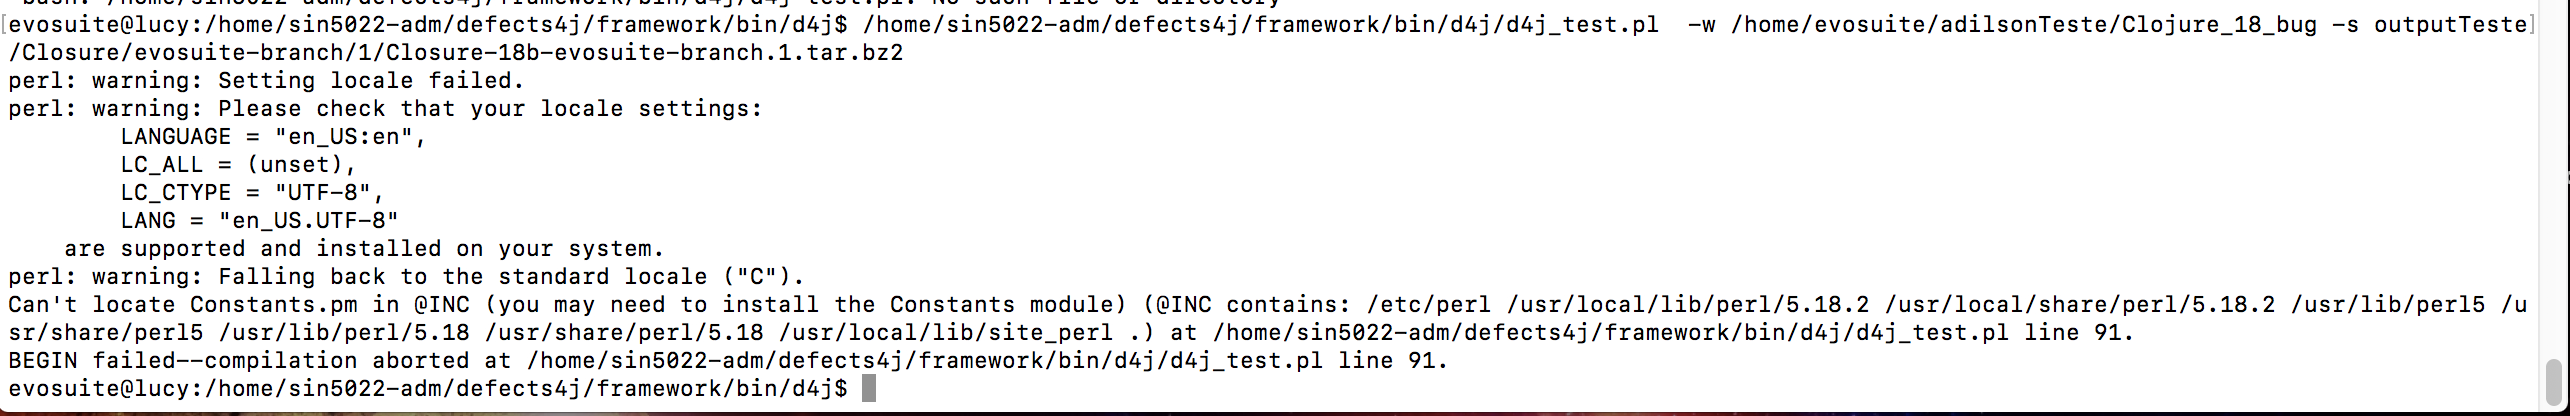
\includegraphics{pic/d4j_testpl.png}
\caption{alt text}
\end{figure}

    Indicando a falta de algumas bibliotecas \emph{Constant module}

    \hypertarget{defects4j-test}{%
\subsubsection{defects4j test}\label{defects4j-test}}

    Ao tentar executar o script: \textbf{defects4j test} com o comando
abaixo:

    \begin{Shaded}
\begin{Highlighting}[]
\ExtensionTok{/home/sin5022-adm/defects4j/framework/bin/defects4j}\NormalTok{ test -w /home/evosuite/adilsonTeste/Clojure_18_bug -s /home/evosuite/adilsonTeste/outputTeste/Closure/evosuite-branch/1/Closure-18b-evosuite-branch.1.tar.bz2}
\end{Highlighting}
\end{Shaded}

    Obtivemos o seguinte erro:

    \begin{figure}
\centering
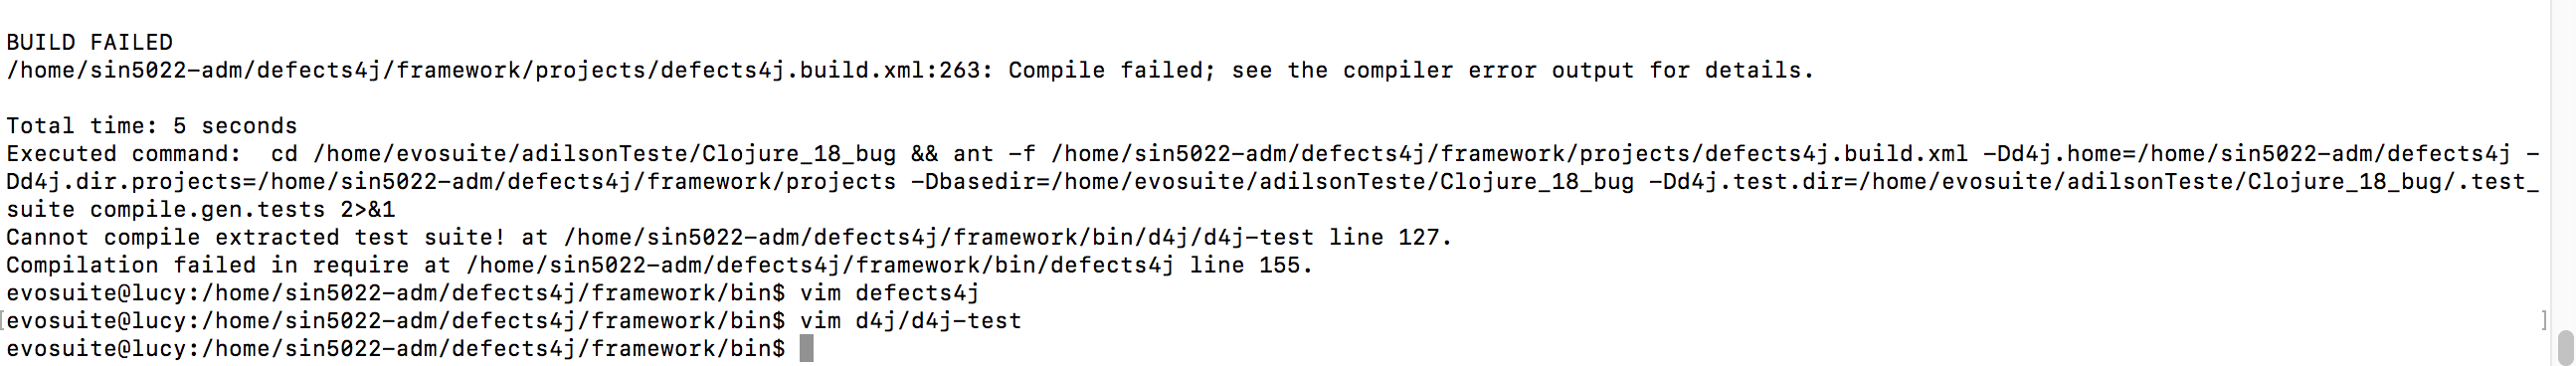
\includegraphics{pic/defects4j_test.png}
\caption{alt text}
\end{figure}

    Indicando que não consegue extrair o casos de teste. Os quais estão no
formato solicitados pela doc
(\href{https://people.cs.umass.edu/~rjust/defects4j/html_doc/d4j/d4j-test.html}{doc\_defects4J})
da ferramenta: \textbf{Closure-18b-evosuite-branch.1.tar.bz2}. De acordo
com essa doc o formato é:
\emph{project\_id-version\_id-test\_suite\_src.test\_id.tar.bz2}

    Seguem alguns exemplos:

\begin{enumerate}
\def\labelenumi{\arabic{enumi}.}
\tightlist
\item
  Lang-11f-randoop.1.tar.bz2
\item
  Lang-12b-evosuite-weakmutation.1.tar.bz2
\item
  Lang-12f-evosuite-branch.1.tar.bz2
\end{enumerate}

    \hypertarget{chamando-junity-na-muxe3o}{%
\section{Chamando Junity na mão}\label{chamando-junity-na-muxe3o}}

    Coloquei os jars do evosuite no classpath do compilador \textbf{javac}
com o comando:

    \begin{Shaded}
\begin{Highlighting}[]
\ExtensionTok{javac}\NormalTok{ -cp .:}\StringTok{"junit-4.12.jar:evosuite-1.0.6.jar"}
\end{Highlighting}
\end{Shaded}

    Em seguida adicionamos o caminho absoluto das classes \textbf{java} que
devem ser compiladas:

    \begin{Shaded}
\begin{Highlighting}[]
\ExtensionTok{javac}\NormalTok{ -cp .:}\StringTok{"junit-4.12.jar:evosuite-1.0.6.jar:"}\NormalTok{ testeJunity/main/java/outropackage/inside1/mult.java testeJunity/main/java/outropackage/ddd.java testeJunity/main/java/projetoCobertura/projetoCobertura/FmtRewrap.java testeJunity/test/java/projetoCobertura/projetoCobertura/FmtRewrapTeste.java}
\end{Highlighting}
\end{Shaded}

    Compilamos, em seguida vamos executar o Junity para a classe de teste
\textbf{projetoCobertura.projetoCobertura.FmtRewrapTeste}:

    \begin{Shaded}
\begin{Highlighting}[]
\ExtensionTok{java}\NormalTok{ -cp .:}\StringTok{"junit-4.12.jar:evosuite-1.0.6.jar:./testeJunity/test/java/:./testeJunity/main/java/"}\NormalTok{ org.junit.runner.JUnitCore projetoCobertura.projetoCobertura.FmtRewrapTeste}
\end{Highlighting}
\end{Shaded}

    Vale ressaltar os seguintes pontos:

\begin{enumerate}
\def\labelenumi{\arabic{enumi}.}
\item
  O nome da classe de teste deve contar apenas o path relativo a classe
  para o projeto e não o caminho absoluto do arquivo no filesystem.
\item
  No classpath adicionamos o Junity, a raiz do projeto onde há o teste,
  a raiz do projeto onde está a classe de teste (ambos em relação ao
  filesystem).
\end{enumerate}

    Segue o output do Junity:

    \begin{figure}
\centering
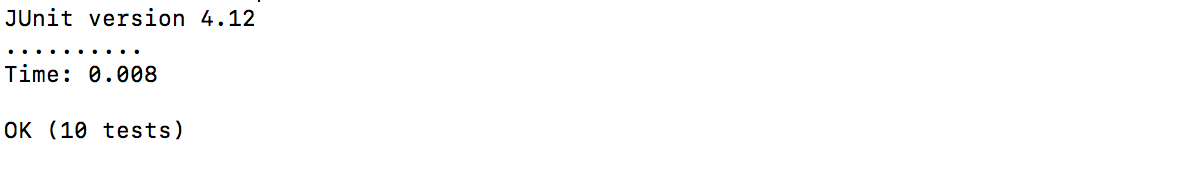
\includegraphics{pic/outputJunity.png}
\caption{alt text}
\end{figure}
Agora vamos executar para o projeto no servidor....
    \hypertarget{observauxe7uxf5es-execuuxe7uxe3o-branch}{%
\section{Observações: execução
branch}\label{observauxe7uxf5es-execuuxe7uxe3o-branch}}

    Vale ressaltar um bug no evosuite que não permite a execução de algumas
classes ao invocar o Junity \(4\) por linha de comando,

    \hypertarget{rodando-mac-os-local-os-testes-unituxe1rios-gerados-no-lucy-para-a-versuxe3o-bug}{%
\subsection{Rodando (MAC OS local) os testes unitários gerados no Lucy
para a versão
bug}\label{rodando-mac-os-local-os-testes-unituxe1rios-gerados-no-lucy-para-a-versuxe3o-bug}}

    Uma classe não compila: \textbf{Graph\_ESTest.java} segue abaixo o erro
de execução encontrado:

    \begin{Shaded}
\begin{Highlighting}[]
\ExtensionTok{javac}\NormalTok{ -cp .:}\StringTok{"junit-4.12.jar:evosuite-1.0.6.jar:./Clojure_18_bug/build/compiler.jar:./outputTeste/Closure/evosuite-branch/1/com/google/javascript/jscomp/"} \VariableTok{$(}\FunctionTok{find}\NormalTok{ outputTeste/Closure/evosuite-branch/1/ -name }\StringTok{"*.java"}\VariableTok{)}
\end{Highlighting}
\end{Shaded}

    \begin{figure}
\centering
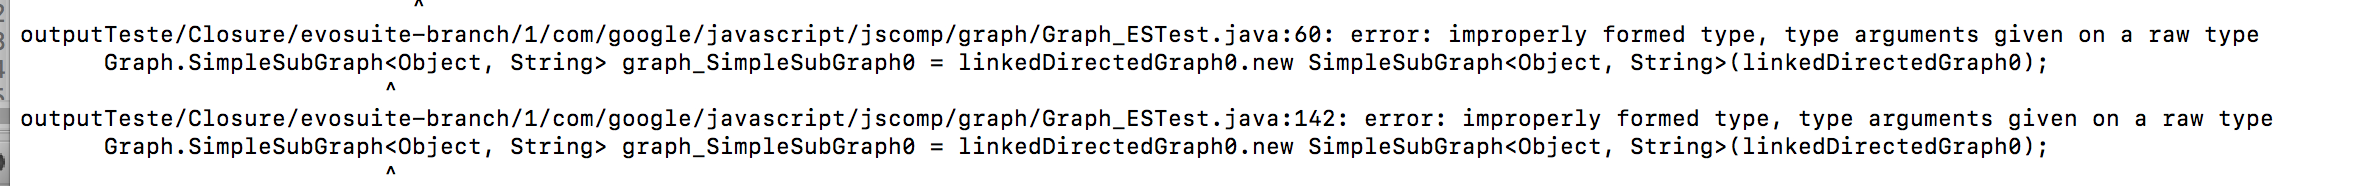
\includegraphics{pic/erroComp.png}
\caption{alt text}
\end{figure}

    Removendo a classe com erro:

    \begin{Shaded}
\begin{Highlighting}[]
\ExtensionTok{--Removi}\NormalTok{ a classe com erro}
\ExtensionTok{javac}\NormalTok{ -cp .:}\StringTok{"junit-4.12.jar:evosuite-1.0.6.jar:./Clojure_18_bug/build/compiler.jar:./outputTeste/Closure/evosuite-branch/1/com/google/javascript/jscomp/"} \VariableTok{$(}\FunctionTok{find}\NormalTok{ outputTeste/Closure/evosuite-branch/1/ -name }\StringTok{"*.java"}\NormalTok{ -and -not -name }\StringTok{"Graph_ESTest.java"}\VariableTok{)}
\end{Highlighting}
\end{Shaded}

    foi possível compilar perfeitamente (\(38\) warnings sobre uso de lib
deprecated). Em seguida, executamos as classes de teste geradas pelo
evosuite!

    \begin{Shaded}
\begin{Highlighting}[]
\ExtensionTok{java}\NormalTok{ -cp .:}\StringTok{"hamcrest-core-1.3.jar:junit-4.12.jar:evosuite-1.0.6.jar:./Clojure_18_bug/build/compiler.jar:./outputTeste/Closure/evosuite-branch/1/"}\NormalTok{ org.junit.runner.JUnitCore com.google.javascript.jscomp.DisambiguateProperties_ESTest com.google.javascript.jscomp.CodingConvention_ESTest com.google.javascript.jscomp.ConstCheck_ESTest com.google.javascript.jscomp.StrictWarningsGuard_ESTest com.google.javascript.jscomp.SyntacticScopeCreator_ESTest com.google.javascript.jscomp.CheckProvides_ESTest com.google.javascript.jscomp.ErrorFormat_ESTest com.google.javascript.jscomp.TypedScopeCreator_ESTest com.google.javascript.jscomp.PassConfig_ESTest com.google.javascript.jscomp.CodingConventions_ESTest com.google.javascript.jscomp.JSModule_ESTest com.google.javascript.jscomp.NodeUtil_ESTest com.google.javascript.jscomp.JsAst_ESTest com.google.javascript.jscomp.DiagnosticGroup_ESTest com.google.javascript.jscomp.CheckGlobalNames_ESTest com.google.javascript.jscomp.CodeChangeHandler_ESTest com.google.javascript.jscomp.PrepareAst_ESTest com.google.javascript.jscomp.JsMessageVisitor_ESTest com.google.javascript.jscomp.CheckGlobalThis_ESTest com.google.javascript.jscomp.CreateSyntheticBlocks_ESTest com.google.javascript.jscomp.TypeValidator_ESTest com.google.javascript.jscomp.DefaultPassConfig_ESTest com.google.javascript.jscomp.JSModuleGraph_ESTest com.google.javascript.jscomp.CodeConsumer_ESTest com.google.javascript.jscomp.StrictModeCheck_ESTest com.google.javascript.jscomp.CrossModuleMethodMotion_ESTest com.google.javascript.jscomp.graph.DiGraph_ESTest com.google.javascript.jscomp.graph.LinkedDirectedGraph_ESTest com.google.javascript.jscomp.AstValidator_ESTest com.google.javascript.jscomp.Normalize_ESTest com.google.javascript.jscomp.TypeCheck_ESTest com.google.javascript.jscomp.LightweightMessageFormatter_ESTest com.google.javascript.jscomp.SourceFile_ESTest com.google.javascript.jscomp.PhaseOptimizer_ESTest com.google.javascript.jscomp.SyntheticAst_ESTest com.google.javascript.jscomp.CheckSideEffects_ESTest com.google.javascript.jscomp.DependencyOptions_ESTest com.google.javascript.jscomp.FunctionTypeBuilder_ESTest com.google.javascript.jscomp.OptimizeCalls_ESTest com.google.javascript.jscomp.SuppressDocWarningsGuard_ESTest com.google.javascript.jscomp.AbstractMessageFormatter_ESTest com.google.javascript.jscomp.Denormalize_ESTest com.google.javascript.jscomp.DiagnosticGroupWarningsGuard_ESTest com.google.javascript.jscomp.ClosureCodingConvention_ESTest com.google.javascript.jscomp.ProcessCommonJSModules_ESTest com.google.javascript.jscomp.CodeGenerator_ESTest com.google.javascript.jscomp.ControlStructureCheck_ESTest com.google.javascript.jscomp.NodeTraversal_ESTest com.google.javascript.jscomp.CheckLevel_ESTest com.google.javascript.jscomp.Compiler_ESTest com.google.javascript.jscomp.type.SemanticReverseAbstractInterpreter_ESTest com.google.javascript.jscomp.type.ChainableReverseAbstractInterpreter_ESTest com.google.javascript.jscomp.GoogleCodingConvention_ESTest com.google.javascript.jscomp.ComposeWarningsGuard_ESTest com.google.javascript.jscomp.ProcessDefines_ESTest com.google.javascript.jscomp.SourceMap_ESTest com.google.javascript.jscomp.Result_ESTest com.google.javascript.jscomp.AbstractCompiler_ESTest com.google.javascript.jscomp.CompilerOptions_ESTest com.google.javascript.jscomp.CleanupPasses_ESTest com.google.javascript.jscomp.DiagnosticType_ESTest com.google.javascript.jscomp.CompilerInput_ESTest com.google.javascript.jscomp.deps.JsFileLineParser_ESTest com.google.javascript.jscomp.deps.JsFileParser_ESTest com.google.javascript.jscomp.deps.SimpleDependencyInfo_ESTest com.google.javascript.jscomp.deps.SortedDependencies_ESTest com.google.javascript.jscomp.DiagnosticGroups_ESTest com.google.javascript.jscomp.WarningsGuard_ESTest com.google.javascript.jscomp.CheckRegExp_ESTest com.google.javascript.jscomp.ControlFlowGraph_ESTest com.google.javascript.jscomp.Scope_ESTest com.google.javascript.jscomp.GlobalNamespace_ESTest com.google.javascript.jscomp.parsing.Config_ESTest com.google.javascript.jscomp.parsing.IRFactory_ESTest com.google.javascript.jscomp.parsing.JsDocInfoParser_ESTest com.google.javascript.jscomp.parsing.ParserRunner_ESTest com.google.javascript.jscomp.parsing.JsDocTokenStream_ESTest com.google.javascript.jscomp.CodePrinter_ESTest com.google.javascript.jscomp.Tracer_ESTest com.google.javascript.jscomp.AnonymousFunctionNamingPolicy_ESTest com.google.javascript.jscomp.MakeDeclaredNamesUnique_ESTest com.google.javascript.jscomp.CheckUnreachableCode_ESTest com.google.javascript.jscomp.CheckDebuggerStatement_ESTest com.google.javascript.jscomp.BasicErrorManager_ESTest com.google.javascript.jscomp.ReplaceIdGenerators_ESTest com.google.javascript.jscomp.PassFactory_ESTest com.google.javascript.jscomp.LoggerErrorManager_ESTest com.google.javascript.jscomp.ProcessTweaks_ESTest com.google.javascript.jscomp.VarCheck_ESTest com.google.javascript.jscomp.CheckAccessControls_ESTest com.google.javascript.jscomp.ReferenceCollectingCallback_ESTest com.google.javascript.jscomp.RhinoErrorReporter_ESTest com.google.javascript.jscomp.JSError_ESTest com.google.javascript.jscomp.VariableReferenceCheck_ESTest com.google.javascript.rhino.ScriptRuntime_ESTest com.google.javascript.rhino.SourcePosition_ESTest com.google.javascript.rhino.IR_ESTest com.google.javascript.rhino.InputId_ESTest com.google.javascript.rhino.JSDocInfo_ESTest com.google.javascript.rhino.JSDocInfoBuilder_ESTest com.google.javascript.rhino.jstype.FunctionParamBuilder_ESTest com.google.javascript.rhino.jstype.StringType_ESTest com.google.javascript.rhino.jstype.ValueType_ESTest com.google.javascript.rhino.jstype.JSTypeRegistry_ESTest com.google.javascript.rhino.jstype.NoType_ESTest com.google.javascript.rhino.jstype.NoResolvedType_ESTest com.google.javascript.rhino.jstype.UnresolvedTypeExpression_ESTest com.google.javascript.rhino.jstype.ProxyObjectType_ESTest com.google.javascript.rhino.jstype.PrototypeObjectType_ESTest com.google.javascript.rhino.jstype.FunctionType_ESTest com.google.javascript.rhino.jstype.NullType_ESTest com.google.javascript.rhino.jstype.NoObjectType_ESTest com.google.javascript.rhino.jstype.FunctionBuilder_ESTest com.google.javascript.rhino.jstype.BooleanType_ESTest com.google.javascript.rhino.jstype.ParameterizedType_ESTest com.google.javascript.rhino.jstype.IndexedType_ESTest com.google.javascript.rhino.jstype.TemplateType_ESTest com.google.javascript.rhino.jstype.ErrorFunctionType_ESTest com.google.javascript.rhino.jstype.UnknownType_ESTest com.google.javascript.rhino.jstype.UnionTypeBuilder_ESTest com.google.javascript.rhino.jstype.JSType_ESTest com.google.javascript.rhino.jstype.NamedType_ESTest com.google.javascript.rhino.jstype.ObjectType_ESTest com.google.javascript.rhino.jstype.AllType_ESTest com.google.javascript.rhino.jstype.NumberType_ESTest com.google.javascript.rhino.jstype.ArrowType_ESTest com.google.javascript.rhino.jstype.UnionType_ESTest com.google.javascript.rhino.jstype.InstanceObjectType_ESTest com.google.javascript.rhino.jstype.VoidType_ESTest com.google.javascript.rhino.Node_ESTest com.google.javascript.rhino.JSTypeExpression_ESTest }\OperatorTok{>}\NormalTok{ resultJunity.txt}
\end{Highlighting}
\end{Shaded}

    Após executar obtivemos \(50\) erros:

    \begin{figure}
\centering

\includegraphics{pic/junit4_evo_testes_sobre_versao_bug.png}
\caption{alt text}
\end{figure}

    \hypertarget{rodando-mac-os-local-os-testes-unituxe1rios-gerados-no-lucy-para-a-versuxe3o-fixed}{%
\subsection{Rodando (MAC OS local) os testes unitários gerados no Lucy
para a versão
fixed}\label{rodando-mac-os-local-os-testes-unituxe1rios-gerados-no-lucy-para-a-versuxe3o-fixed}}

    A compilação dos testes para a versão fixed usa o mesmo comando
alterando apenas um parâmetro (o jar da versão fixed ao invés da versão
bug dentro do classpath):

    \begin{Shaded}
\begin{Highlighting}[]
\ExtensionTok{javac}\NormalTok{ -cp .:}\StringTok{"junit-4.12.jar:evosuite-1.0.6.jar:./Clojure_18_fixed/build/compiler.jar:./outputTeste/Closure/evosuite-branch/1/com/google/javascript/jscomp/"} \VariableTok{$(}\FunctionTok{find}\NormalTok{ outputTeste/Closure/evosuite-branch/1/ -name }\StringTok{"*.java"}\VariableTok{)}
\end{Highlighting}
\end{Shaded}

    Uma classe não compila: \textbf{Graph\_ESTest.java} segue abaixo o erro
de execução encontrado (como na execução de cima):

    \begin{figure}
\centering
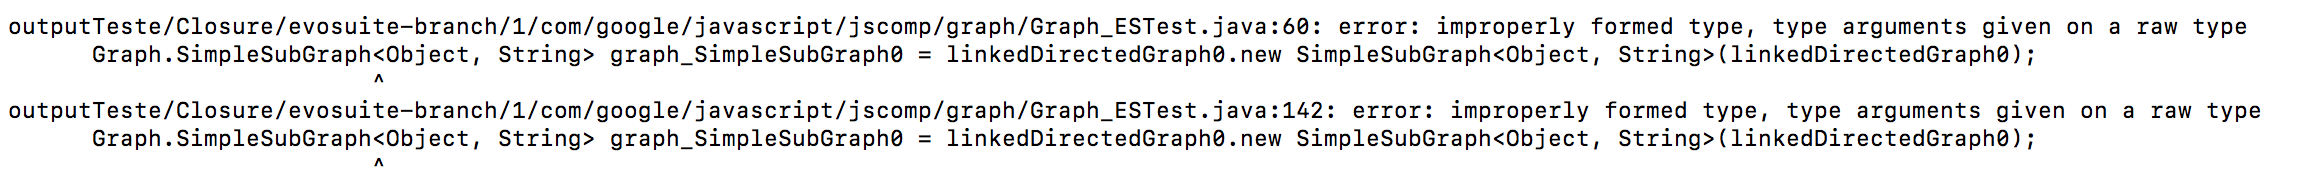
\includegraphics{pic/erroCompFixed.png}
\caption{alt text}
\end{figure}

    Removendo a classe com erro:

    \begin{Shaded}
\begin{Highlighting}[]
\ExtensionTok{--Removi}\NormalTok{ a classe com erro}
\ExtensionTok{javac}\NormalTok{ -cp .:}\StringTok{"junit-4.12.jar:evosuite-1.0.6.jar:./Clojure_18_fixed/build/compiler.jar:./outputTeste/Closure/evosuite-branch/1/com/google/javascript/jscomp/"} \VariableTok{$(}\FunctionTok{find}\NormalTok{ outputTeste/Closure/evosuite-branch/1/ -name }\StringTok{"*.java"}\NormalTok{ -and -not -name }\StringTok{"Graph_ESTest.java"}\VariableTok{)}
\end{Highlighting}
\end{Shaded}

    foi possível compilar perfeitamente (\(38\) warnings sobre uso de lib
deprecated). Em seguida, executamos as classes de teste geradas pelo
evosuite!

    \begin{Shaded}
\begin{Highlighting}[]
\ExtensionTok{java}\NormalTok{ -cp .:}\StringTok{"hamcrest-core-1.3.jar:junit-4.12.jar:evosuite-1.0.6.jar:./Clojure_18_fixed/build/compiler.jar:./outputTeste/Closure/evosuite-branch/1/"}\NormalTok{ org.junit.runner.JUnitCore com.google.javascript.jscomp.DisambiguateProperties_ESTest com.google.javascript.jscomp.CodingConvention_ESTest com.google.javascript.jscomp.ConstCheck_ESTest com.google.javascript.jscomp.StrictWarningsGuard_ESTest com.google.javascript.jscomp.SyntacticScopeCreator_ESTest com.google.javascript.jscomp.CheckProvides_ESTest com.google.javascript.jscomp.ErrorFormat_ESTest com.google.javascript.jscomp.TypedScopeCreator_ESTest com.google.javascript.jscomp.PassConfig_ESTest com.google.javascript.jscomp.CodingConventions_ESTest com.google.javascript.jscomp.JSModule_ESTest com.google.javascript.jscomp.NodeUtil_ESTest com.google.javascript.jscomp.JsAst_ESTest com.google.javascript.jscomp.DiagnosticGroup_ESTest com.google.javascript.jscomp.CheckGlobalNames_ESTest com.google.javascript.jscomp.CodeChangeHandler_ESTest com.google.javascript.jscomp.PrepareAst_ESTest com.google.javascript.jscomp.JsMessageVisitor_ESTest com.google.javascript.jscomp.CheckGlobalThis_ESTest com.google.javascript.jscomp.CreateSyntheticBlocks_ESTest com.google.javascript.jscomp.TypeValidator_ESTest com.google.javascript.jscomp.DefaultPassConfig_ESTest com.google.javascript.jscomp.JSModuleGraph_ESTest com.google.javascript.jscomp.CodeConsumer_ESTest com.google.javascript.jscomp.StrictModeCheck_ESTest com.google.javascript.jscomp.CrossModuleMethodMotion_ESTest com.google.javascript.jscomp.graph.DiGraph_ESTest com.google.javascript.jscomp.graph.LinkedDirectedGraph_ESTest com.google.javascript.jscomp.AstValidator_ESTest com.google.javascript.jscomp.Normalize_ESTest com.google.javascript.jscomp.TypeCheck_ESTest com.google.javascript.jscomp.LightweightMessageFormatter_ESTest com.google.javascript.jscomp.SourceFile_ESTest com.google.javascript.jscomp.PhaseOptimizer_ESTest com.google.javascript.jscomp.SyntheticAst_ESTest com.google.javascript.jscomp.CheckSideEffects_ESTest com.google.javascript.jscomp.DependencyOptions_ESTest com.google.javascript.jscomp.FunctionTypeBuilder_ESTest com.google.javascript.jscomp.OptimizeCalls_ESTest com.google.javascript.jscomp.SuppressDocWarningsGuard_ESTest com.google.javascript.jscomp.AbstractMessageFormatter_ESTest com.google.javascript.jscomp.Denormalize_ESTest com.google.javascript.jscomp.DiagnosticGroupWarningsGuard_ESTest com.google.javascript.jscomp.ClosureCodingConvention_ESTest com.google.javascript.jscomp.ProcessCommonJSModules_ESTest com.google.javascript.jscomp.CodeGenerator_ESTest com.google.javascript.jscomp.ControlStructureCheck_ESTest com.google.javascript.jscomp.NodeTraversal_ESTest com.google.javascript.jscomp.CheckLevel_ESTest com.google.javascript.jscomp.Compiler_ESTest com.google.javascript.jscomp.type.SemanticReverseAbstractInterpreter_ESTest com.google.javascript.jscomp.type.ChainableReverseAbstractInterpreter_ESTest com.google.javascript.jscomp.GoogleCodingConvention_ESTest com.google.javascript.jscomp.ComposeWarningsGuard_ESTest com.google.javascript.jscomp.ProcessDefines_ESTest com.google.javascript.jscomp.SourceMap_ESTest com.google.javascript.jscomp.Result_ESTest com.google.javascript.jscomp.AbstractCompiler_ESTest com.google.javascript.jscomp.CompilerOptions_ESTest com.google.javascript.jscomp.CleanupPasses_ESTest com.google.javascript.jscomp.DiagnosticType_ESTest com.google.javascript.jscomp.CompilerInput_ESTest com.google.javascript.jscomp.deps.JsFileLineParser_ESTest com.google.javascript.jscomp.deps.JsFileParser_ESTest com.google.javascript.jscomp.deps.SimpleDependencyInfo_ESTest com.google.javascript.jscomp.deps.SortedDependencies_ESTest com.google.javascript.jscomp.DiagnosticGroups_ESTest com.google.javascript.jscomp.WarningsGuard_ESTest com.google.javascript.jscomp.CheckRegExp_ESTest com.google.javascript.jscomp.ControlFlowGraph_ESTest com.google.javascript.jscomp.Scope_ESTest com.google.javascript.jscomp.GlobalNamespace_ESTest com.google.javascript.jscomp.parsing.Config_ESTest com.google.javascript.jscomp.parsing.IRFactory_ESTest com.google.javascript.jscomp.parsing.JsDocInfoParser_ESTest com.google.javascript.jscomp.parsing.ParserRunner_ESTest com.google.javascript.jscomp.parsing.JsDocTokenStream_ESTest com.google.javascript.jscomp.CodePrinter_ESTest com.google.javascript.jscomp.Tracer_ESTest com.google.javascript.jscomp.AnonymousFunctionNamingPolicy_ESTest com.google.javascript.jscomp.MakeDeclaredNamesUnique_ESTest com.google.javascript.jscomp.CheckUnreachableCode_ESTest com.google.javascript.jscomp.CheckDebuggerStatement_ESTest com.google.javascript.jscomp.BasicErrorManager_ESTest com.google.javascript.jscomp.ReplaceIdGenerators_ESTest com.google.javascript.jscomp.PassFactory_ESTest com.google.javascript.jscomp.LoggerErrorManager_ESTest com.google.javascript.jscomp.ProcessTweaks_ESTest com.google.javascript.jscomp.VarCheck_ESTest com.google.javascript.jscomp.CheckAccessControls_ESTest com.google.javascript.jscomp.ReferenceCollectingCallback_ESTest com.google.javascript.jscomp.RhinoErrorReporter_ESTest com.google.javascript.jscomp.JSError_ESTest com.google.javascript.jscomp.VariableReferenceCheck_ESTest com.google.javascript.rhino.ScriptRuntime_ESTest com.google.javascript.rhino.SourcePosition_ESTest com.google.javascript.rhino.IR_ESTest com.google.javascript.rhino.InputId_ESTest com.google.javascript.rhino.JSDocInfo_ESTest com.google.javascript.rhino.JSDocInfoBuilder_ESTest com.google.javascript.rhino.jstype.FunctionParamBuilder_ESTest com.google.javascript.rhino.jstype.StringType_ESTest com.google.javascript.rhino.jstype.ValueType_ESTest com.google.javascript.rhino.jstype.JSTypeRegistry_ESTest com.google.javascript.rhino.jstype.NoType_ESTest com.google.javascript.rhino.jstype.NoResolvedType_ESTest com.google.javascript.rhino.jstype.UnresolvedTypeExpression_ESTest com.google.javascript.rhino.jstype.ProxyObjectType_ESTest com.google.javascript.rhino.jstype.PrototypeObjectType_ESTest com.google.javascript.rhino.jstype.FunctionType_ESTest com.google.javascript.rhino.jstype.NullType_ESTest com.google.javascript.rhino.jstype.NoObjectType_ESTest com.google.javascript.rhino.jstype.FunctionBuilder_ESTest com.google.javascript.rhino.jstype.BooleanType_ESTest com.google.javascript.rhino.jstype.ParameterizedType_ESTest com.google.javascript.rhino.jstype.IndexedType_ESTest com.google.javascript.rhino.jstype.TemplateType_ESTest com.google.javascript.rhino.jstype.ErrorFunctionType_ESTest com.google.javascript.rhino.jstype.UnknownType_ESTest com.google.javascript.rhino.jstype.UnionTypeBuilder_ESTest com.google.javascript.rhino.jstype.JSType_ESTest com.google.javascript.rhino.jstype.NamedType_ESTest com.google.javascript.rhino.jstype.ObjectType_ESTest com.google.javascript.rhino.jstype.AllType_ESTest com.google.javascript.rhino.jstype.NumberType_ESTest com.google.javascript.rhino.jstype.ArrowType_ESTest com.google.javascript.rhino.jstype.UnionType_ESTest com.google.javascript.rhino.jstype.InstanceObjectType_ESTest com.google.javascript.rhino.jstype.VoidType_ESTest com.google.javascript.rhino.Node_ESTest com.google.javascript.rhino.JSTypeExpression_ESTest }\OperatorTok{>}\NormalTok{ resultJunity.txt}
\end{Highlighting}
\end{Shaded}

    Após executar obtivemos \(51\) erros:

    \begin{figure}
\centering
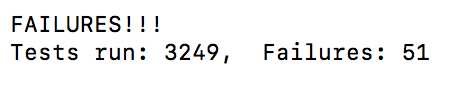
\includegraphics{pic/junit4_evo_testes_sobre_versao_fixed.png}
\caption{alt text}
\end{figure}

    \hypertarget{next-steps}{%
\section{Next steps}\label{next-steps}}

    \begin{enumerate}
\def\labelenumi{\arabic{enumi}.}
\tightlist
\item
  Analisar os 101 erros de ambas as execuções, comparar as duas
  (intersecção)
\item
  Avaliar qual é o erro extra encontrado
\item
  Avaliar se o erro faz sentido, ou não
\end{enumerate}


    % Add a bibliography block to the postdoc
    
    
    
    \end{document}
